% !TeX root = ../../Book1.tex
% 纲要标题：## 第4章　拓扑空间、商构造与局部—整体工具
% 纲要位置：几何学计划纲要.md，第 234 行。
% 正文状态：初稿；尚未正式审核。

% 纲要内容开始
% 
% > 本章目标与证明范围：为后续流形和商空间建立足够的一般拓扑。基本定义在同一构造中连续出现；较深部分集中在分离性、局部有限性、度量化和单位分解，而非平均分配给每个名词。
% 
% 纲要内容结束

\chapter{拓扑空间、商构造与局部—整体工具}
\label{g1:ch:04}
\BookChapterNumber{g1:ch:04}

\begin{chapterabstract}
	拓扑记录邻近关系与连续变化，使空间不必先以某个 Euclid 空间中的子集出现。子空间、积与商分别处理限制、同时记录和识别；紧性与连通性帮助辨认这些构造保留了什么。为了把局部 Euclid 模型组织成可操作的整体，还需要分离性、可数性和局部有限性。本章证明局部紧第二可数 Hausdorff 空间的仿紧性、正则第二可数空间的度量化，以及仿紧 Hausdorff 空间上连续单位分解的存在，并用环面、实射影空间与两个非分离商模型核验这些条件。
\end{chapterabstract}

\begin{learninggoals}
	\begin{itemize}
		\item 用开集、拓扑基和连续映射描述子空间、积空间及商空间，逐项检查映射的下降与泛性质。
		\item 使用紧性证明最值与同胚判据，区分连通、道路连通和局部道路连通，判断分支在映射下如何变化。
		\item 从局部紧性与第二可数性构造紧穷竭和局部有限细化，说明 Hausdorff、正则与正规条件在证明中的不同作用。
		\item 构造分离闭集的连续函数，并由可数函数族建立与原拓扑相容的距离。
		\item 从覆盖收缩与截断函数构造单位分解，粘合连续函数和正定型，同时识别不能直接加权的条件。
		\item 完整核验环面与实射影空间的商模型，利用双原点和稠密轨道商说明局部形式不保证整体分离性。
	\end{itemize}
\end{learninggoals}

把线段 \([0,1]\) 的两个端点识别成一个点，会得到圆周。这个说法在图形上很直观，但如果只把 \(0\) 与 \(1\) 规定为同一个等价类，还没有说明新空间中的“附近”是什么意思。特别是粘合点附近的一小段圆弧，在原线段中会分成靠近两端的两小段。映射
\[
	q:[0,1]\longrightarrow S^1,\qquad q(t)=(\cos2\pi t,\sin2\pi t)
\]
提示了合适的判断：圆周中的一个集合应当开，当且仅当它在原线段中的原像开。这样既保留了参数的连续变化，也给识别点规定了正确的邻域。

\ProseParagraphBreak

同样的任务会在几何中反复出现。一个圆柱可以由长方形的一对边识别得到，第二章中的实射影空间可以由球面的对径点识别得到；局部坐标又要求我们把空间的一小块同 Euclid 开集相比较。但是识别过程有时会让不同点无法用不交邻域分开，局部公式也可能在无限多个区域聚集的地方失去连续性。分离性控制点能否由邻域区分，局部有限性控制无穷多份局部数据怎样在每点附近相加；紧性与可数性使这些控制能够在全空间上组织起来。

\ProseParagraphBreak

本章从开集出发建立这些工具。所需基础是集合的并、交、原像与等价关系，实数的完备性、闭有界区间的紧性、连续实函数的基本性质，以及有限维线性代数。Euclid 空间中的开球与极限会作为具体模型；一般空间中的紧性以开覆盖定义，序列刻画则在具备相应条件时使用。关于基础构造与紧性的进一步阅读，可参看 Lee 的正式第二版\cite[第2章, 第19--37页; 第3章, 第49--80页; 第4章, 第86--117页]{Lee2011Topological}，其中分离性与可数性、商空间、局部紧性和仿紧性按相应主题展开。本章所用的度量化和单位分解均在正文证明，光滑截断函数则在光滑流形的微积分工具中继续构造。

% !TeX root = ../../Book1.tex
% 纲要标题：### 4.1 拓扑与映射的基本构造
% 纲要位置：几何学计划纲要.md，第 238 行。
% 正文状态：初稿完成；尚未正式审核。

% 纲要内容开始
% 
% * 度量拓扑、拓扑基及连续性
% * 子空间、积空间与映射的泛性质
% * 商拓扑、粘合及商映射的检验
% * 同胚不变量与商空间的反例
% 
% 纲要内容结束

\section{拓扑与映射的基本构造}
\label{g1:sec:0401}

在平面中判断一条曲线是否连续，可以测量点的距离；把曲线的两个端点识别后，距离公式却未必还合用。我们仍希望知道哪些点足够接近、原来的连续映射何时能通过识别后的空间。开集提供了一套能同时处理这两种情形的语言。本节始终把构造空间与检验映射放在一起：子空间和积空间适合检验映入的映射，商空间适合检验从它映出的映射。

\subsection{度量拓扑、拓扑基及连续性}
\label{g1:subsec:0401:01}

Euclid 开球有两个与具体半径无关的性质：开集的任意并仍开，有限个开集的交仍开。第二个条件只能要求有限交，例如实直线上的开区间 \((-1/m,1/m)\) 的交是单点集 \(\{0\}\)。我们把这两项性质保留下来，允许点附近的形状由问题决定。

\begin{definition}[拓扑空间]\label{g1:def:topology}
	设 \(X\) 为集合。若其子集族 \(\mathcal T\) 含 \(\varnothing,X\)，对任意并和有限交封闭，则称 \(\mathcal T\) 为 \(X\) 上的一个\term[tuopu]{拓扑}[topology]，称 \((X,\mathcal T)\) 为\term[tuopukongjian]{拓扑空间}[topological space]。\(\mathcal T\) 中的集合称为\term[kaiji]{开集}[open set]，开集的补集称为\term[biji]{闭集}[closed set]。若 \(N\subseteq X\) 包含一个含 \(x\) 的开集，则称 \(N\) 为 \(x\) 的\term[linyu]{邻域}[neighborhood]。
\end{definition}

邻域本身不必开；“开邻域”才同时要求开性。由补集运算，任意闭集的交和有限闭集的并仍闭。\(\varnothing\) 与 \(X\) 既开又闭，因此“开”与“闭”并非互相排斥的两种分类。一个集合也可以既不开又不闭，例如通常实直线中的 \([0,1)\)。

对 \(A\subseteq X\)，所有包含于 \(A\) 的开集之并称为它的\term[neibu]{内部}[interior]，记为 \(\operatorname{Int}_X A\)；所有包含 \(A\) 的闭集之交称为它的\term[bibao]{闭包}[closure]，记为 \(\overline A^{\,X}\)，环境明确时省去上标。它们分别是包含于 \(A\) 的最大开集和包含 \(A\) 的最小闭集。集合 \(\overline A\setminus\operatorname{Int}_X A\) 称为 \(A\) 的\term[bianjie]{边界}[boundary]，记为 \(\partial_X A\)。这里的边界由所在空间决定；同一子集放入较小的环境，边界可能改变。

\begin{proposition}[闭包的邻域判据]\label{g1:prop:closure-neighborhood}
	设 \(A\) 为拓扑空间 \(X\) 的子集。点 \(x\) 属于 \(\overline A\)，当且仅当 \(x\) 的每个开邻域都与 \(A\) 相交。此外，
	\[
		X\setminus\overline A=\operatorname{Int}_X(X\setminus A).
	\]
\end{proposition}
\begin{proof}
	若 \(x\notin\overline A\)，则开集 \(X\setminus\overline A\) 是一个不交 \(A\) 的邻域。反之，若存在含 \(x\) 的开集 \(U\) 与 \(A\) 不交，则闭集 \(X\setminus U\) 包含 \(A\)，所以 \(\overline A\subseteq X\setminus U\)，特别是 \(x\notin\overline A\)。这个判据同时说明，\(x\notin\overline A\) 等价于它属于 \(X\setminus A\) 中的某个开集，给出所写等式。
\end{proof}

若 \(\overline A=X\)，称 \(A\) 在 \(X\) 中\term[choumi]{稠密}[dense]。由刚才的判据，这等价于 \(A\) 与每个非空开集相交；有理数在通常实直线中稠密，就是这一条件的熟悉例子。

度量是产生拓扑的一种重要方式，但不是拓扑定义的一部分。

\begin{definition}[度量及其拓扑]\label{g1:def:metric-topology}
	设 \(X\) 为集合。若函数 \(d:X\times X\to[0,\infty)\) 对所有 \(x,y,z\in X\) 都满足
	\[
		d(x,y)=0\Longleftrightarrow x=y,\qquad d(x,y)=d(y,x),\qquad d(x,z)\le d(x,y)+d(y,z),
	\]
	则称这个函数为\term[duliang]{度量}[metric]。记 \(B_d(x,r)=\{y:d(x,y)<r\}\)，其中 \(r>0\)。规定 \(U\subseteq X\) 开，当且仅当每个 \(x\in U\) 都有 \(r>0\) 使 \(B_d(x,r)\subseteq U\)；所得拓扑称为 \(d\) 的\term[duliangtuopu]{度量拓扑}[metric topology]。
\end{definition}

这确实给出拓扑：并集中的点已经落在某一个成员中，可沿用该成员提供的球；有限交中的点可取有限个正半径的最小值。每个球本身也开，因为若 \(y\in B_d(x,r)\)，则三角不等式给出
\[
	B_d\bigl(y,r-d(x,y)\bigr)\subseteq B_d(x,r).
\]
前三章使用的 Euclid 距离就是这个定义的例子。另一个例子是离散度量：不同点的距离都取 \(1\)。此时每个单点都是半径 \(1/2\) 的球，所有子集都开；这一拓扑称为\term[lisantuopu]{离散拓扑}[discrete topology]。在另一端，只有 \(\varnothing,X\) 开的拓扑称为\term[pingfantuopu]{平凡拓扑}[indiscrete topology]。当 \(X\) 至少有两个点时，平凡拓扑不能来自度量，因为度量总能用足够小的球区分不同点。

\begin{definition}[拓扑基]\label{g1:def:topological-basis}
	设 \(X\) 为拓扑空间，\(\mathcal B\) 是它的一族开集。若对任意开集 \(U\) 和 \(x\in U\)，都存在 \(B\in\mathcal B\) 使 \(x\in B\subseteq U\)，则称这族开集为一个\term[tuopuji]{拓扑基}[topological basis]。等价地，每个开集都是若干基元素的并。
\end{definition}

基把“检查所有开集”缩减为“检查一批足够小的开集”。度量空间的全体开球构成基；实直线中有理端点的开区间也构成基，因为每个开区间内部的点都能夹在两个合适的有理数之间。

\begin{proposition}[从集合族产生拓扑]\label{g1:prop:basis-test}
	设 \(\mathcal B\) 为集合 \(X\) 的子集族。它是某个拓扑的基，当且仅当它覆盖 \(X\)，并且对任意 \(B_1,B_2\in\mathcal B\) 及 \(x\in B_1\cap B_2\)，存在 \(B_3\in\mathcal B\) 使 \(x\in B_3\subseteq B_1\cap B_2\)。此时全体基元素的并组成唯一的相应拓扑。
\end{proposition}
\begin{proof}
	若已经是拓扑基，覆盖性质来自开集 \(X\)，交集条件来自开集 \(B_1\cap B_2\)。反过来，把所有基元素的并组成的集合族记为 \(\mathcal T\)。空并是 \(\varnothing\)，覆盖条件给出 \(X\in\mathcal T\)，任意并显然仍在 \(\mathcal T\) 中。若 \(x\in U\cap V\)，其中 \(U,V\in\mathcal T\)，可先找含 \(x\) 的基元素 \(B_1\subseteq U\)、\(B_2\subseteq V\)，再由假设找到 \(B_3\subseteq U\cap V\)。因此 \(U\cap V\) 也是基元素的并。有限交由归纳得到，故 \(\mathcal T\) 为拓扑，且 \(\mathcal B\) 是它的基。任何以 \(\mathcal B\) 为基的拓扑都必须由这些并组成，所以唯一。
\end{proof}

\begin{definition}[连续映射]\label{g1:def:continuous-map}
	设 \(f:X\to Y\) 为拓扑空间之间的映射。若每个开集 \(V\subseteq Y\) 的原像 \(f^{-1}(V)\) 都在 \(X\) 中开，则称其为\term[lianxuyingshe]{连续映射}[continuous map]。
\end{definition}

这个定义也可只在目标的一组基上检验，因为原像保持任意并。它等价于闭集的原像闭；还等价于逐点条件：对每个 \(x\in X\) 及 \(f(x)\) 的开邻域 \(V\)，存在 \(x\) 的开邻域 \(U\)，使 \(f(U)\subseteq V\)。确实，连续时可取 \(U=f^{-1}(V)\)；反之，各点提供的 \(U\) 把 \(f^{-1}(V)\) 表成开集的并。在度量空间中把 \(V\) 取为 \(\varepsilon\)-球，并在 \(U\) 中取一个 \(\delta\)-球，就恢复了分析学中的 \(\varepsilon\)--\(\delta\) 条件。

在一般拓扑空间中，给定序列 \((x_m)\)。如果 \(x\) 的每个开邻域都包含该序列从某一项起的全部项，就称该序列\term[shoulian]{收敛}[converge]于 \(x\)，记为 \(x_m\to x\)。连续映射保持这种收敛：若 \(x_m\to x\)，则对 \(f(x)\) 的每个开邻域 \(V\)，连续性使 \(f^{-1}(V)\) 成为 \(x\) 的开邻域，因而最终 \(x_m\in f^{-1}(V)\)，即最终 \(f(x_m)\in V\)。所以 \(f(x_m)\to f(x)\)。

恒等映射连续，两个连续映射的复合连续，因为 \((g\circ f)^{-1}(V)=f^{-1}(g^{-1}(V))\)。但一般连续映射不把开集映成开集：常值映射 \(\mathbb R\to\mathbb R\) 已是反例。把每个开集都映成开集的映射称为\term[kaiyingshe]{开映射}[open map]；类似定义\term[biyingshe]{闭映射}[closed map]。连续性检验的是原像，开映射、闭映射检验的是像，三个条件不能混用。

\begin{definition}[同胚]\label{g1:def:homeomorphism}
	双射 \(f:X\to Y\) 若与逆映射 \(f^{-1}:Y\to X\) 都连续，则称为\term[tongpei]{同胚}[homeomorphism]。存在同胚的两个空间称为同胚的，记为 \(X\cong Y\)。
\end{definition}

对连续双射，逆映射连续等价于原映射开，也等价于原映射闭。这不是额外定理：逆映射对于集合的原像正是原映射对于该集合的像。因而证明一个显式双射是同胚时，既可以写出逆映射并检查连续性，也可以证明开性或闭性。

\subsection{子空间、积空间与映射的泛性质}
\label{g1:subsec:0401:02}

圆周 \(S^1=\{(x,y)\in\mathbb R^2:x^2+y^2=1\}\) 上的开集通常不是平面开集：一小段圆弧在平面内没有面积，却应当是圆周上的开集。若把对象放在一个已有空间中，就应把环境的开集限制到这个对象上。

设 \(A\subseteq X\)。集合族 \(\{A\cap U:U\subseteq X\text{ 开}\}\) 在 \(A\) 上组成拓扑，称为\term[zikongjiantuopu]{子空间拓扑}[subspace topology]。公理直接来自交集与并、交运算的相容性。这个定义还说明：子空间 \(A\) 中的闭集恰为 \(A\cap F\)，其中 \(F\) 在 \(X\) 中闭。例如 \([0,1)\) 在子空间 \([0,1]\) 中开，因为它等于 \([0,1]\cap(-1,1)\)；它并不在 \(\mathbb R\) 中开。

\begin{proposition}[子空间的映入判据]\label{g1:prop:subspace-universal}
	设 \(A\subseteq X\) 带子空间拓扑，\(i:A\hookrightarrow X\) 为包含映射。对任意拓扑空间 \(Z\) 及集合映射 \(f:Z\to A\)，\(f\) 连续当且仅当 \(i\circ f\) 连续。
\end{proposition}
\begin{proof}
	包含映射连续，因为 \(i^{-1}(U)=A\cap U\)。所以 \(f\) 连续时复合连续。反过来，若 \(i\circ f\) 连续，则对 \(A\) 中开集 \(A\cap U\)，有 \(f^{-1}(A\cap U)=(i\circ f)^{-1}(U)\)，故原像开。
\end{proof}

这一性质把子空间拓扑与映射的目标联系起来：给定连续映射 \(g:Z\to X\)，若它的像包含于 \(A\)，就存在唯一的连续映射 \(f:Z\to A\) 使下图交换。
\[
	\begin{tikzcd}[column sep=large,row sep=large]
		& A \arrow[d,hook,"i"] \\
		Z \arrow[ur,dashed,"f"] \arrow[r,"g"'] & X
	\end{tikzcd}
\]
这里“唯一”来自集合映射的取值已经被 \(g\) 决定；拓扑保证这个唯一的映射连续。这类用存在唯一映射来刻画构造的性质称为\term[fanxingzhi]{泛性质}[universal property]。

积空间处理的是把几个量同时记录下来。对拓扑空间 \(X,Y\)，全体开矩形 \(U\times V\) 满足\cref{g1:prop:basis-test}，由它们生成的拓扑称为 \(X\times Y\) 的\term[jituopu]{积拓扑}[product topology]。有限个空间的积同样以 \(\prod_{i=1}^mU_i\) 为基。对任意指标集 \(I\)，积 \(\prod_{i\in I}X_i\) 的基本开集则规定为
\begin{equation}\label{g1:eq:product-basic-open}
	\bigcap_{i\in F}\pi_i^{-1}(U_i),\qquad F\subseteq I\text{ 有限},\quad U_i\subseteq X_i\text{ 开},
\end{equation}
其中 \(\pi_i\) 是第 \(i\) 个坐标投影。也就是说，一次只限制有限个坐标，其余坐标任取。交两个这样的集合仍只限制有限个坐标，所以确实给出一组基。

\begin{proposition}[积空间的映入判据]\label{g1:prop:product-universal}
	设 \((X_i)_{i\in I}\) 为拓扑空间族，积空间取上述积拓扑。映射 \(f:Z\to\prod_iX_i\) 连续，当且仅当每个坐标映射 \(f_i=\pi_i\circ f\) 连续。因此给定连续映射族 \(f_i:Z\to X_i\)，存在唯一的连续映射 \(f\) 满足 \(\pi_i\circ f=f_i\)。
\end{proposition}
\begin{proof}
	投影 \(\pi_i\) 连续，因为 \(\pi_i^{-1}(U_i)\) 是基本开集。故 \(f\) 连续时各坐标连续。反过来，对\eqref{g1:eq:product-basic-open}中的基本开集，其原像为有限交 \(\bigcap_{i\in F}f_i^{-1}(U_i)\)，所以开。存在唯一的集合映射由 \(f(z)=(f_i(z))_i\) 给出，刚才的判据保证连续。
\end{proof}

有限积的图示为
\[
	\begin{tikzcd}[column sep=large,row sep=large]
		& Z \arrow[dl,"f_1"'] \arrow[d,dashed,"f"] \arrow[dr,"f_2"] & \\
		X_1 & X_1\times X_2 \arrow[l,"\pi_1"] \arrow[r,"\pi_2"'] & X_2 .
	\end{tikzcd}
\]
如果在无限积中允许每个坐标都受一个开集限制，所得的是通常更细的盒拓扑，逐坐标连续就不再够用。例如 \(t\mapsto(t,t,\ldots)\) 从 \(\mathbb R\) 到 \(\mathbb R^{\mathbb N}\) 的所有坐标都连续，而集合 \(\prod_{n\ge1}(-1/n,1/n)\) 的原像是不开的 \(\{0\}\)。这个集合在盒拓扑中开，在积拓扑中并不开：任何含零序列的基本开集只限制有限个坐标，不能保证其余坐标满足所写不等式。

有限个度量空间 \((X_i,d_i)\) 的积拓扑由度量
\[
	D(x,y)=\max_{1\le i\le m}d_i(x_i,y_i)
\]
产生。三角不等式逐坐标成立，再取最大值即可；\(D\)-球是相同半径的开球之积，而每个含 \(x\) 的基本开矩形都包含某个这样的球。因此有限积既能用坐标也能用距离来理解。连续映射在子集上的限制仍连续，这由包含映射连续和复合连续立即得到。

\subsection{商拓扑、粘合及商映射的检验}
\label{g1:subsec:0401:03}

现在把问题倒过来。若 \(q:X\to Y\) 已经规定哪些点要合并，如何给 \(Y\) 选拓扑？目标是使“合并后的一块区域开”能够在原来的空间中检查。由于这块区域可能包含多个代表，必须同时检查它的全部原像，而不能只挑一份代表。

\begin{definition}[商拓扑与商映射]\label{g1:def:quotient-map}
	设 \(q:X\to Y\) 为从拓扑空间到集合的满射。规定
	\[
		U\subseteq Y\text{ 开}\quad\Longleftrightarrow\quad q^{-1}(U)\subseteq X\text{ 开},
	\]
	得到的拓扑称为由 \(q\) 给出的\term[shangtuopu]{商拓扑}[quotient topology]。若 \(Y\) 已有拓扑，且满射 \(q\) 满足这个等价关系，则称 \(q\) 为\term[shangyingshe]{商映射}[quotient map]。当 \(Y=X/{\sim}\) 是等价类的集合且 \(q(x)=[x]\) 时，所得空间称为\term[shangkongjian]{商空间}[quotient space]。
\end{definition}

原像保持任意并和有限交，故上述定义确实满足拓扑公理。商映射必连续；进一步说，商拓扑是使 \(q\) 连续的最细拓扑，因为任何这样的拓扑中的开集都必须有开原像。若 \(A\subseteq X\) 是一些完整等价类的并，即 \(q^{-1}(q(A))=A\)，称它为\term[baoheji]{饱和集}[saturated set]。商空间的开集与原空间的饱和开集一一对应。

\begin{proposition}[映射从商空间下降]\label{g1:prop:quotient-descent}
	设 \(q:X\to Y\) 为商映射，\(Z\) 为拓扑空间。集合映射 \(h:Y\to Z\) 连续，当且仅当 \(h\circ q\) 连续。特别地，若连续映射 \(f:X\to Z\) 在 \(q\) 的每个纤维上取常值，则存在唯一连续映射 \(\bar f:Y\to Z\)，使 \(f=\bar f\circ q\)。
\end{proposition}
\begin{proof}
	一个方向来自复合连续。另一个方向中，对 \(Z\) 的开集 \(V\)，等式
	\[
		q^{-1}\bigl(h^{-1}(V)\bigr)=(h\circ q)^{-1}(V)
	\]
	说明左侧开，再由商映射的判据得到 \(h^{-1}(V)\) 开。若 \(f\) 在纤维上常值，就可定义 \(\bar f(y)=f(x)\)，其中任选 \(q(x)=y\)；纤维上的常值性使选择无关，满射性保证定义处处成立且唯一，连续性由刚证的判据得到。
\end{proof}

下降的图示为
\[
	\begin{tikzcd}[column sep=large,row sep=large]
		X \arrow[r,"f"] \arrow[d,two heads,"q"'] & Z \\
		Y \arrow[ur,dashed,"\bar f"'] &
	\end{tikzcd}
\]
它把构造分成两个实质条件：纤维常值保证映射良定义，商拓扑保证连续。只写一个代表元公式而不检验第一项，就还没有得到商空间上的映射。

\begin{proposition}[商映射的实用判据]\label{g1:prop:quotient-tests}
	连续满射 \(q:X\to Y\) 若为开映射或闭映射，则为商映射。若 \(q\) 是商映射，\(U\subseteq Y\) 开，则限制 \(q:q^{-1}(U)\to U\) 仍为商映射。
\end{proposition}
\begin{proof}
	只需补证“原像开蕴含目标开”。若 \(q\) 开且 \(q^{-1}(V)\) 开，满射性给出 \(V=q(q^{-1}(V))\) 开。若 \(q\) 闭，则 \(q^{-1}(Y\setminus V)\) 闭，其像 \(Y\setminus V\) 闭，所以 \(V\) 开。

	对限制的结论，\(q^{-1}(U)\) 在 \(X\) 中开。若 \(V\subseteq U\) 的原像在 \(q^{-1}(U)\) 中开，它也在 \(X\) 中开，故 \(V\) 在 \(Y\) 中开，因而在 \(U\) 中开；相反方向由限制连续得到。
\end{proof}

开映射和闭映射只是充分条件。实际工作中也可以直接找一组饱和开集来描述商拓扑。尤其要注意，连续满射只能保证“目标开蕴含原像开”，还缺反方向。例如把带离散拓扑的 \(\mathbb R\) 恒等映到带通常拓扑的 \(\mathbb R\)，是连续满射，却不是商映射。

粘合是商构造的一个常见来源。给定空间 \(X,Y\)，先取它们的\term[bujiaobing]{不交并}[disjoint union] \(X\sqcup Y\)：点保留来自哪一份的标签，一个集合开当且仅当它与每一份的交开。给定 \(A\subseteq X\) 及连续映射 \(a:A\to Y\)，再取由关系 \(x\sim a(x)\)（\(x\in A\)）生成的等价关系，得到粘合空间 \(X\cup_aY\)。这里“生成”包括传递性所迫使的所有识别；若 \(a\) 非单射，\(A\) 中不同的点也可能合并。根据下降判据，给定连续映射 \(f_X:X\to Z\)、\(f_Y:Y\to Z\)，它们恰在
\[
	f_X|_A=f_Y\circ a
\]
时粘成唯一连续映射 \(X\cup_aY\to Z\)。这条等式就是粘合处必须满足的相容条件。

另一个方向是：一个空间已经由若干子空间覆盖，能否从各片上的连续性推出整体连续性？需要对覆盖加条件。

\begin{proposition}[粘合引理]\label{g1:prop:gluing-lemma}
	设 \(X=\bigcup_{\alpha\in I}A_\alpha\)，且每个 \(A_\alpha\) 带子空间拓扑。假设或者所有 \(A_\alpha\) 都在 \(X\) 中开，或者 \(I\) 有限且所有 \(A_\alpha\) 都在 \(X\) 中闭。若连续映射 \(f_\alpha:A_\alpha\to Y\) 在交集上两两相同，则它们定义唯一连续映射 \(f:X\to Y\)。
\end{proposition}
\begin{proof}
	交集上的相等性使 \(f(x)=f_\alpha(x)\) 与所选覆盖成员无关，覆盖性保证处处有定义，也给出唯一性。开覆盖情形，对开集 \(V\subseteq Y\)，每个 \(f_\alpha^{-1}(V)\) 在 \(A_\alpha\) 中开，因 \(A_\alpha\) 在 \(X\) 中开，它也在 \(X\) 中开；这些集合的并是 \(f^{-1}(V)\)，所以开。有限闭覆盖情形改用闭集 \(F\subseteq Y\)：\(f_\alpha^{-1}(F)\) 在 \(A_\alpha\) 中闭，因 \(A_\alpha\) 在 \(X\) 中闭，它也在 \(X\) 中闭；有限并 \(f^{-1}(F)\) 仍闭，故 \(f\) 连续。
\end{proof}

例如 \(|x|\) 由两个闭半轴上的公式 \(-x\)、\(x\) 粘成，它们在交点 \(0\) 处一致。有限闭覆盖的“有限”不能删去，因为闭集的任意并不一定闭；习题给出各片均有非空区间的具体反例。后面局部有限覆盖所起的作用之一，正是恢复这种闭集并的控制。

\subsection{同胚不变量与商空间的反例}
\label{g1:subsec:0401:04}

同胚只保留由开集表达的结构。距离、角度、面积不在其中，例如 \(x\mapsto2x\) 是 \(\mathbb R^n\) 的同胚，却改变长度。与此相对，能否把两个不同的点放进不相交的开邻域，是只涉及开集的问题。

\begin{definition}[Hausdorff 空间]\label{g1:def:hausdorff}
	设 \(X\) 为拓扑空间。若任意不同的点 \(x,y\in X\) 都有不相交的开邻域 \(U\ni x\)、\(V\ni y\)，则称它为\term[Hausdorffkongjian]{Hausdorff 空间}[Hausdorff space]。\footnote{Felix Hausdorff（1868--1942），德国数学家，对一般拓扑、集合论及维数理论作出重要贡献。}
\end{definition}

度量空间都是 Hausdorff 的：若 \(d(x,y)=r>0\)，两个半径 \(r/3\) 的球若相交，三角不等式就给出 \(r<2r/3\)，矛盾。子空间继承 Hausdorff 性，因为可把两个不交的环境开邻域与子空间相交；任意积也继承这一性质，因为两个不同的点必在某一坐标不同，拉回该坐标中分离它们的两个开集即可。

若 \(h:X\to Y\) 为同胚且 \(X\) 为 Hausdorff 空间，则 \(Y\) 中不同两点的原像能被不交开集分离，而这两个开集在 \(h\) 下的像仍开，因此 \(Y\) 也为 Hausdorff 空间。像这样在同胚下保持的性质称为\term[tongpeibubianliang]{同胚不变量}[topological invariant]。后面引入的紧性与连通性也将给出不变量；它们有用，是因为一旦发现不变量不同，就能排除所有可能的同胚，而不必逐一尝试公式。

\begin{example}[连续双射不一定是同胚]\label{g1:exm:half-open-circle}
	给 \([0,1)\) 通常的子空间拓扑，给 \(S^1\subseteq\mathbb C\cong\mathbb R^2\) 子空间拓扑。映射
	\[
		f:[0,1)\longrightarrow S^1,\qquad f(t)=e^{2\pi it}
	\]
	连续且为双射，但不是同胚。事实上，\([0,1/4)\) 在 \([0,1)\) 中开，而它的像包含 \(1\)，却不含任何角度为负且足够接近 \(0\) 的圆周点。每个 \(1\) 的圆周开邻域都包含这样的点，所以该像不开。因而 \(f^{-1}\) 不连续。
\end{example}

这个例子的两个空间都来自 Euclid 空间，问题仍会发生。连续双射允许把原来相距很远的端部压到相邻位置，逆映射因此可能把一个很小的邻域撕开。\cref{g1:thm:compact-bijection}将给出一个常用补救：若源空间紧、目标空间 Hausdorff，连续双射就必为同胚。

\begin{example}[合并点可以破坏分离性]\label{g1:exm:two-point-quotient}
	在通常实直线中保留原点为一个等价类，把所有非零点合并为另一个等价类。商集合记为 \(\{a,b\}\)，其中 \(a=[0]\)。单点集 \(\{b\}\) 的原像是开集 \(\mathbb R\setminus\{0\}\)，而 \(\{a\}\) 的原像 \(\{0\}\) 不开，所以商拓扑恰为
	\[
		\{\varnothing,\{b\},\{a,b\}\}.
	\]
	含 \(a\) 的唯一开邻域是整个空间，因此 \(a,b\) 不能被不交开邻域分离。源空间为 Hausdorff 空间，商空间却不是。
\end{example}

所以“把某些点看成同一点”只确定了商构造的输入，并不自动保证结果是通常想象中的几何空间。后面处理环面与实射影空间时，我们会分别核验等价类、连续性与分离性；双原点和有理平移的商则显示这些核验分别可能在哪里失败。

% !TeX root = ../../Book1.tex
% 纲要标题：### 4.2 紧性、连通性与局部条件
% 纲要位置：几何学计划纲要.md，第 245 行。
% 正文状态：初稿完成；未送审。

% 纲要内容开始
% 
% * 紧性与有限交性质
% * 局部紧性与相对紧邻域
% * 连通、道路连通与局部道路连通
% * 分支及其在映射下的行为
% 
% 纲要内容结束

\section{紧性、连通性与局部条件}
\label{g1:sec:0402}

在第三章，单位球面的紧性使一列法向量留下极限方向；有限 Helly 定理却不能直接处理无穷多个约束，因为可行点可能不断逃向远处。本节把这些现象放到一般拓扑空间中：紧性让任意开覆盖缩减为有限覆盖，连通性则排除把空间分成两个互不接触的开部分。两者解决不同问题。局部紧性只要求在每一点附近保留紧性；局部道路连通性则保证足够小的邻域里能够用道路连接点。它们将把后文的局部坐标和整体构造联系起来。

\subsection{紧性与有限交性质}
\label{g1:subsec:0402:01}

设 \(K\subseteq X\)。一个由 \(X\) 的开集组成的族 \(\{U_\alpha\}_{\alpha\in A}\) 若满足 \(K\subseteq\bigcup_{\alpha\in A}U_\alpha\)，就称为 \(K\) 的开覆盖。这里的指标集不必可数，覆盖中的集合也不必彼此不同。

\begin{definition}[紧性与有限交性质]\label{g1:def:compact}
	若拓扑空间 \(X\) 的每个开覆盖都有有限子覆盖，则称 \(X\) 为\term[jinkongjian]{紧空间}[compact space]。若子集 \(K\subseteq X\) 在子空间拓扑下是紧空间，就称其为\term[jinji]{紧集}[compact set]；等价地，\(X\) 中每个覆盖 \(K\) 的开集族都有有限子族覆盖 \(K\)。

	若集合族 \(\{F_\alpha\}_{\alpha\in A}\) 中每个有限子族的交都非空，就称它具有\term[youxianjiaoxingzhi]{有限交性质}[finite intersection property]；空子族的交约定为整个所在空间。
\end{definition}

上述子集定义的等价性来自子空间开集的形式 \(K\cap U\)：把子空间中的覆盖写成这种形式，有限子覆盖的选取与环境空间中的覆盖完全对应。空集是紧集；有限集也紧，因为给每个点选一个覆盖它的开集便已足够。

\ProseParagraphBreak

本章的“紧”只表示开覆盖性质，不暗含 Hausdorff 条件；需要分离性时会在陈述中另列。部分文献把同一开覆盖性质称为\term[nijin]{拟紧}[quasi-compact]，并把“紧”保留给拟紧且 Hausdorff 的空间。读到这类资料时须先转换约定。后文的流形本身要求 Hausdorff，届时两种用法在流形的紧子集上没有差别。

\begin{theorem}[紧性的闭集刻画]\label{g1:thm:compact-fip}
	拓扑空间 \(X\) 紧，当且仅当 \(X\) 的每个具有有限交性质的闭集族都有非空交集。
\end{theorem}
\begin{proof}
	设 \(X\) 紧，而闭集族 \(\{F_\alpha\}\) 具有有限交性质。若全交为空，则补集族 \(\{X\setminus F_\alpha\}\) 是开覆盖。由紧性取有限子覆盖，取补集便得到某个有限子族的交为空，与假设矛盾。

	反之，设每个具有有限交性质的闭集族都有公共点。若开覆盖 \(\{U_\alpha\}\) 没有有限子覆盖，则对任意有限个指标 \(\alpha_1,\ldots,\alpha_m\)，都有
	\[
		\bigcap_{j=1}^m(X\setminus U_{\alpha_j})
		=X\setminus\bigcup_{j=1}^mU_{\alpha_j}\ne\varnothing.
	\]
	因此补集闭族具有有限交性质，应该有公共点，但这个点不属于任何 \(U_\alpha\)，与开覆盖矛盾。若 \(X=\varnothing\)，空覆盖已有有限子覆盖，而约定排除了在空空间中具有有限交性质的族，两种刻画仍然一致。
\end{proof}

这一表述把“有限次约束可解”与“全部约束同时可解”接上了。闭性不能删除：\((0,1/n)\) 是紧空间 \([0,1]\) 的子集，任意有限个相交非空，全交却为空，因为这些子集没有保留趋近端点的极限。紧性也不能删除：\([n,\infty)\) 是 \(\mathbb R\) 中的闭集，有限交非空，全交为空。这正是\cref{g1:exm:helly-infinite-family}中的两个失败机制。

\begin{proposition}[闭子集与有限并]\label{g1:prop:compact-closed-subset}
	紧空间的闭子集是紧集。任意拓扑空间中，有限个紧子集的并仍紧。
\end{proposition}
\begin{proof}
	若 \(F\) 闭于紧空间 \(X\)，给定 \(F\) 的一个环境开覆盖，把 \(X\setminus F\) 加入后便覆盖 \(X\)。取有限子覆盖，再删去 \(X\setminus F\)，得到原覆盖中有限个集合覆盖 \(F\)。

	若 \(K_1,\ldots,K_m\) 都紧，给定它们的并的开覆盖，对每个 \(K_j\) 各取一个有限子覆盖，再合并这 \(m\) 个有限族即可。
\end{proof}

\begin{proposition}[紧集的连续像]\label{g1:prop:compact-image}
	若 \(f:X\to Y\) 连续且 \(K\subseteq X\) 紧，则 \(f(K)\) 是 \(Y\) 的紧子集；这里不要求 \(X,Y\) 为 Hausdorff 空间。
\end{proposition}
\begin{proof}
	给定 \(f(K)\) 的开覆盖 \(\{V_\alpha\}\)，由连续性，\(\{f^{-1}(V_\alpha)\}\) 是覆盖 \(K\) 的开集族。取有限子覆盖后，对应的有限个 \(V_\alpha\) 就覆盖 \(f(K)\)。
\end{proof}

\begin{proposition}[紧集在 Hausdorff 空间中闭]\label{g1:prop:compact-hausdorff-closed}
	若 \(Y\) 为 Hausdorff 空间，\(K\subseteq Y\) 紧，则 \(K\) 闭于 \(Y\)。
\end{proposition}
\begin{proof}
	只需对每个 \(y\in Y\setminus K\) 找到与 \(K\) 不交的开邻域。若 \(K=\varnothing\)，没有需要证明的内容。否则，对每个 \(x\in K\)，Hausdorff 条件给出开集 \(U_x,V_x\)，分别含 \(x,y\)，且 \(U_x\cap V_x=\varnothing\)。从覆盖 \(K\) 的 \(\{U_x\}_{x\in K}\) 中取有限子覆盖 \(U_{x_1},\ldots,U_{x_m}\)，则
	\[
		V=V_{x_1}\cap\cdots\cap V_{x_m}
	\]
	是 \(y\) 的开邻域，并与覆盖 \(K\) 的每个 \(U_{x_j}\) 不交。因此 \(V\cap K=\varnothing\)，证明 \(Y\setminus K\) 开。
\end{proof}

连续实函数在非空紧空间上取得最大值和最小值。事实上，若 \(X\) 非空且紧、\(f:X\rightarrow\mathbb R\) 连续，由\cref{g1:prop:compact-image}，\(f(X)\) 是非空紧子集；由上一命题它在 \(\mathbb R\) 中闭。开区间族 \(\{(-n,n)\}_{n\ge1}\) 覆盖 \(f(X)\)，紧性给出有限子覆盖，所以 \(f(X)\) 还有界。实数完备性给出其上、下确界，它们都是 \(f(X)\) 的极限点或已在其中的点，闭性保证二者属于 \(f(X)\)。因此确有原像取得这两个最值。

这里 Hausdorff 条件先分开一对点，紧性再把所有这些局部分离合并为一次有限交。若没有分离性，结论会失败：两点集 \(\{a,b\}\) 取拓扑 \(\{\varnothing,\{a\},\{a,b\}\}\)，单点 \(\{a\}\) 紧，却不闭，因为其补集 \(\{b\}\) 不开。

\begin{theorem}[由紧性判定同胚]\label{g1:thm:compact-bijection}
	若 \(X\) 紧、\(Y\) 为 Hausdorff 空间，且 \(f:X\to Y\) 是连续双射，则 \(f\) 是同胚。
\end{theorem}
\begin{proof}
	双射已经给出了集合映射 \(f^{-1}:Y\to X\)，只需证明它连续。对任意闭集 \(F\subseteq X\)，\cref{g1:prop:compact-closed-subset}给出 \(F\) 紧；其连续像 \(f(F)\) 紧，由 \(Y\) 为 Hausdorff 及\cref{g1:prop:compact-hausdorff-closed}知 \(f(F)\) 闭。注意这里的 \(f(F)\) 正是映射 \(f^{-1}\) 对 \(F\) 的原像。因此逆映射对闭集取原像仍为闭集，也就连续。
\end{proof}

这一判据常用于参数化和粘合空间：连续性与双射容易直接核对，逆映射却不容易写出。紧性和 Hausdorff 条件让逆映射的连续性自动跟上。条件确有作用：连续双射 \(t\mapsto(\cos2\pi t,\sin2\pi t)\) 从 \([0,1)\) 到圆周不是同胚，原因是在圆周上趋近 \((1,0)\) 的点既可对应趋近 \(0\) 的参数，也可对应趋近 \(1\) 的参数；定义域不紧。若定义域取两点离散空间、值域取同一集合上的平凡拓扑，则恒等映射是从紧空间出发的连续双射，逆映射却不连续；此时值域不是 Hausdorff。

\begin{proposition}[有限积的紧性]\label{g1:prop:finite-product-compact}
	有限个紧拓扑空间的积在积拓扑下紧，不要求各因子为 Hausdorff。
\end{proposition}
\begin{proof}
	只需证明两个紧空间 \(X,Y\) 的积紧，再归纳。若任一因子为空，积为空。设两者非空，给定 \(X\times Y\) 的开覆盖 \(\mathcal U\)。积拓扑的开矩形是基：对每个 \((x,y)\)，可选开矩形 \(A_{x,y}\times B_{x,y}\) 含 \((x,y)\)，并使它包含在某个 \(U_{x,y}\in\mathcal U\) 中。

	先固定 \(x\)。开集族 \(\{B_{x,y}\}_{y\in Y}\) 覆盖 \(Y\)，由 \(Y\) 紧，可选 \(y_1,\ldots,y_m\) 使相应的 \(B_{x,y_j}\) 覆盖 \(Y\)。令
	\[
		A_x=\bigcap_{j=1}^m A_{x,y_j}.
	\]
	这是 \(x\) 的开邻域，而且整个 \(A_x\times Y\) 都被有限个 \(U_{x,y_j}\) 覆盖：给定 \((a,b)\)，先选 \(j\) 使 \(b\in B_{x,y_j}\)，而 \(a\in A_x\subseteq A_{x,y_j}\)。

	再让 \(x\) 变化。由 \(X\) 紧，从覆盖 \(\{A_x\}_{x\in X}\) 中选有限子覆盖 \(A_{x_1},\ldots,A_{x_r}\)。对每个 \(x_i\) 保留上一步的有限个 \(U_{x_i,y_j}\)，把它们合并便覆盖 \(X\times Y\)。有限个因子的结论逐次应用这一证明得到；空积约定为单点空间，也紧。
\end{proof}

有限积证明两次使用紧性：先沿一条“纤维”找到有限个覆盖片，再把这个有限选择保持到纤维附近，最后沿另一因子再取有限次。它只处理有限个因子，没有据此证明任意无限积的紧性。在 Euclid 空间中，本书已使用的基本分析结论“闭且有界当且仅当紧”与这里的开覆盖定义相符；但一般拓扑空间没有范数，也没有可供替代定义的“有界”概念。

\subsection{局部紧性与相对紧邻域}
\label{g1:subsec:0402:02}

\(\mathbb R^n\) 本身不紧，任一点却都藏在一个闭球的内部，而闭球紧。后文常只需在一个给定区域内处理数据，希望先把关注的紧集包进一个稍大的开集，再使这个开集的闭包仍然紧且不碰到区域外部。这样既留下调整数据的空间，又保留紧集上的有限性。

\begin{definition}[局部紧性]\label{g1:def:locally-compact}
	设 \(X\) 为拓扑空间。若每个 \(x\in X\) 都有紧邻域，即存在紧集 \(N\subseteq X\) 和开集 \(O\)，使 \(x\in O\subseteq N\)，则称该空间是\term[jubujin]{局部紧}[locally compact]的。若子集 \(A\subseteq X\) 的闭包 \(\overline A\) 紧，则称 \(A\) 为\term[xiangduijin]{相对紧}[relatively compact]的。
\end{definition}

紧邻域本身未必开。定义只先给出一个紧邻域，而几何构造往往需要在任意指定的小邻域内选择这样的对象。对 Hausdorff 空间，这一步可以做到；证明先处理紧空间内部的缩小。

\begin{lemma}[紧 Hausdorff 空间中的邻域缩小]\label{g1:lem:compact-hausdorff-shrink}
	若 \(X\) 为紧 Hausdorff 空间，\(G\subseteq X\) 开且 \(x\in G\)，则存在开集 \(V\)，使
	\[
		x\in V\subseteq\overline V\subseteq G.
	\]
\end{lemma}
\begin{proof}
	令 \(F=X\setminus G\)。它是紧空间的闭子集，因而紧。若 \(F=\varnothing\)，取 \(V=X\)。否则，对每个 \(y\in F\)，由 Hausdorff 条件选不交开集 \(P_y,Q_y\)，分别含 \(x,y\)。有限个 \(Q_{y_1},\ldots,Q_{y_m}\) 覆盖 \(F\)。取
	\[
		V=\bigcap_{j=1}^mP_{y_j},\qquad Q=\bigcup_{j=1}^mQ_{y_j}.
	\]
	则 \(V\) 开且含 \(x\)，而 \(V\subseteq X\setminus Q\)。后者是闭集，所以 \(\overline V\subseteq X\setminus Q\subseteq X\setminus F=G\)。
\end{proof}

\begin{lemma}[局部紧 Hausdorff 空间中的邻域缩小]\label{g1:lem:local-compact-shrink}
	设 \(X\) 为局部紧 Hausdorff 空间，\(x\in U\subseteq X\)，其中 \(U\) 开。则存在开集 \(V\)，使 \(x\in V\)、\(\overline V\) 紧，且 \(\overline V\subseteq U\)。
\end{lemma}
\begin{proof}
	取 \(x\) 的紧邻域 \(N\) 及开集 \(O\)，满足 \(x\in O\subseteq N\)。由 Hausdorff 条件和\cref{g1:prop:compact-hausdorff-closed}，\(N\) 闭于 \(X\)；它作为子空间仍为 Hausdorff。于是 \(N\) 是紧 Hausdorff 空间，\(G=O\cap U\) 是 \(N\) 中含 \(x\) 的开集。

	在 \(N\) 中应用上一引理，得到 \(N\) 中的开集 \(W\)，满足 \(x\in W\subseteq\overline W^{\,N}\subseteq G\)。写 \(W=N\cap H\)，其中 \(H\) 开于 \(X\)。由于 \(W\subseteq G\subseteq O\subseteq N\)，有
	\[
		W=H\cap O.
	\]
	因此 \(W\) 实际上也开于 \(X\)。又因 \(N\) 闭，\(X\) 中的闭包 \(\overline W^{\,X}\) 包含在 \(N\) 内，恰等于 \(\overline W^{\,N}\)。它是紧空间 \(N\) 的闭子集，因而紧，并包含在 \(G\subseteq U\) 中。取 \(V=W\) 即可。
\end{proof}

这说明在 Hausdorff 条件下，局部紧性等价于“每点都有由相对紧开集组成的邻域基”。这里的闭包必须在原空间 \(X\) 中取。只说某个较小子空间内的闭包紧，不能自动控制它在 \(X\) 中还会增加哪些边界点。

\begin{proposition}[紧集的相对紧开邻域]\label{g1:prop:compact-neighborhood-shrink}
	设 \(X\) 为局部紧 Hausdorff 空间，\(K\subseteq X\) 紧，且 \(U\subseteq X\) 是含 \(K\) 的开集。则存在开集 \(V\)，使
	\[
		K\subseteq V\subseteq\overline V\subseteq U,\qquad \overline V\text{ 紧}.
	\]
\end{proposition}
\begin{proof}
	若 \(K=\varnothing\)，取 \(V=\varnothing\)。否则，对每个 \(x\in K\)，由\cref{g1:lem:local-compact-shrink}选开邻域 \(V_x\)，使 \(\overline{V_x}\) 紧且包含在 \(U\) 中。紧性给出有限个 \(V_{x_1},\ldots,V_{x_m}\) 覆盖 \(K\)。令 \(V=\bigcup_{j=1}^mV_{x_j}\)。有限并与闭包相容，所以
	\[
		\overline V=\bigcup_{j=1}^m\overline{V_{x_j}}\subseteq U.
	\]
	右边的有限个紧集之并紧，故 \(\overline V\) 紧。
\end{proof}

这里必须先取有限子覆盖再取并。无限多个相对紧开集的并未必相对紧，例如 \(\bigcup_{m\ge1}(-m,m)=\mathbb R\)。对后续构造，命题给出了两层余地：\(K\) 在 \(V\) 的内部，而 \(\overline V\) 仍留在 \(U\) 内。若一个连续函数最终被构造成在 \(X\setminus V\) 上为零，那么其非零点集的闭包就包含在紧集 \(\overline V\) 中；这正是控制支撑所需的几何条件。如何构造这种函数，还需下一节的分离工具，不能仅由集合包含关系推出。

\ProseParagraphBreak

Euclid 空间以及它的开子集局部紧：在给定点与给定开邻域中选一个足够小的闭球即可。更一般地，若一个 Hausdorff 空间每点附近都同胚于 \(\mathbb R^n\) 的开子集，就可以把小闭球经逆坐标映射送回来；连续像保持紧性，而开球的像提供内部邻域，因此这种空间局部紧。这一论证将直接适用于后文的拓扑流形。相比之下，\(\mathbb Q\) 取实直线诱导的拓扑时并不局部紧，相关极限缺失将在习题中具体说明。

\subsection{连通、道路连通与局部道路连通}
\label{g1:subsec:0402:03}

在直线中，从一个点连续移动到另一点必须经过中间位置；但一般空间的连通性先只排除“分成两块”，并不承诺存在可以行走的参数曲线。这两个要求需要分别定义。

\begin{definition}[连通与道路连通]\label{g1:def:connected-path-connected}
	若拓扑空间 \(X\) 不能写成两个非空、不交开集的并，则称它\term[liantong]{连通}[connected]。这样的并分解若存在，称为 \(X\) 的一个分离。等价地，\(X\) 中同时开且闭的子集只有 \(\varnothing,X\)。子集的连通性总指其子空间拓扑。

	从 \(x\in X\) 到 \(y\in X\) 的一条\term[daolu]{道路}[path]是连续映射 \(\gamma:[0,1]\to X\)，满足 \(\gamma(0)=x\)、\(\gamma(1)=y\)。若任意两点间都有道路，则称 \(X\)\term[daoluliantong]{道路连通}[path-connected]。
\end{definition}

空空间按上述定义既连通又道路连通。以后谈某点所在的分支时，空间当然含有该点。开闭子集刻画是因为分离 \(X=U\sqcup V\) 同时使 \(U\) 的补集 \(V\) 开；反过来，非空真开闭子集与其补集就给出分离。

\begin{lemma}[区间的连通性]\label{g1:lem:interval-connected}
	实直线的每个区间都连通。
\end{lemma}
\begin{proof}
	若区间 \(I=A\sqcup B\) 是分离，选 \(a\in A,b\in B\)，必要时交换两者，使 \(a<b\)。因为 \(I\) 是区间，\([a,b]\subseteq I\)。令 \(c=\sup(A\cap[a,b])\)。集合 \(A\) 在 \(I\) 中既开又闭，而上确界性质表明 \(c\) 属于 \(A\cap[a,b]\) 的闭包，故 \(c\in A\)。特别地，\(c\ne b\)，因为 \(b\in B\)。于是 \(c<b\)，由 \(A\) 在 \(I\) 中开，可在 \(c\) 的右边找到仍属于 \(A\cap[a,b]\) 的点，与 \(c\) 为上确界矛盾。
\end{proof}

\begin{proposition}[连续像、闭包与相交的连通集]\label{g1:prop:connected-image-closure}
	拓扑空间中有下列结论。
	\begin{enumerate}
		\item 连通空间在连续映射下的像连通。
		\item 若 \(A\) 连通且 \(A\subseteq B\subseteq\overline A\)，则 \(B\) 连通；特别是 \(\overline A\) 连通。
		\item 若一族连通子集 \(\{C_\alpha\}\) 有公共点，则它们的并连通。
	\end{enumerate}
\end{proposition}
\begin{proof}
	若 \(f(X)\) 有分离，把两个相对开部分取原像，就会得到 \(X\) 的两个非空、不交开集，它们的并为 \(X\)，与 \(X\) 连通矛盾。这证明第一项。

	对第二项，\(A=\varnothing\) 时，\(B=\varnothing\)，结论成立。否则，假设 \(B=U\sqcup V\) 是分离。把分离限制到 \(A\)，连通性迫使 \(A\) 全在其中一侧，不妨 \(A\subseteq U\)。取 \(v\in V\)。由 \(V\) 在 \(B\) 中开，可写 \(V=B\cap O\)，其中 \(O\) 开于环境空间且含 \(v\)。但 \(v\in B\subseteq\overline A\)，由闭包的邻域刻画，\(O\cap A\ne\varnothing\)；又因 \(A\subseteq B\)，这意味着 \(V\cap A\ne\varnothing\)，矛盾。

	对第三项，固定公共点 \(p\)。若 \(\bigcup_\alpha C_\alpha=U\sqcup V\) 是分离，不妨 \(p\in U\)。每个 \(C_\alpha\) 都连通且遇到 \(U\)，因而不能再遇到 \(V\)，于是所有 \(C_\alpha\subseteq U\)，迫使 \(V=\varnothing\)，矛盾。
\end{proof}

\begin{corollary}\label{g1:cor:path-connected-connected}
	道路连通空间连通，且道路连通空间的连续像仍道路连通。
\end{corollary}
\begin{proof}
	若道路连通空间 \(X\) 有分离 \(X=U\sqcup V\)，取两侧的点及连接它们的道路 \(\gamma\)。由\cref{g1:lem:interval-connected}和上一命题，\(\gamma([0,1])\) 连通，却同时遇到分离的两侧，矛盾。若 \(f:X\to Y\) 连续，给定像中的两点，选它们在 \(X\) 中的原像，再把连接原像的道路与 \(f\) 复合，就得到像中的道路。
\end{proof}

例如 Euclid 空间中的凸集道路连通，因为 \(\gamma(t)=(1-t)x+ty\) 始终位于该集合中。连通性允许的形状更广，它不要求两点间的线段留在集合里，甚至不保证存在任何道路。下面的例子把这一区别落实到一个平面紧集。

\begin{example}[拓扑正弦曲线]\label{g1:exm:topologist-sine}
	令
	\[
		G=\{(x,\sin(1/x)):0<x\le1\},\qquad I_0=\{0\}\times[-1,1],\qquad S=G\cup I_0.
	\]
	集合 \(S\) 称为\term[tuopuzhengxianquxian]{拓扑正弦曲线}[topologist's sine curve]。集合 \(G\) 是区间 \((0,1]\) 在连续映射 \(x\mapsto(x,\sin(1/x))\) 下的像，所以连通且道路连通。其在 \(\mathbb R^2\) 中的闭包恰为 \(S\)。一方面，正横坐标处图像的极限仍由连续函数给出，横坐标为零时纵坐标只能落在 \([-1,1]\)。另一方面，对任意 \(y\in[-1,1]\)，选 \(\theta\) 使 \(\sin\theta=y\)，则对充分大的整数 \(n\)，
	\[
		x_n=(2\pi n+\theta)^{-1}>0,\qquad (x_n,\sin(1/x_n))=(x_n,y)\longrightarrow(0,y).
	\]
	因此 \(I_0\subseteq\overline G\)。由\cref{g1:prop:connected-image-closure}，\(S=\overline G\) 连通；它闭且有界，故也是平面中的紧集。

	不过，没有道路能从 \(I_0\) 到达 \(G\)。假设存在这样的道路，写为 \(\gamma(t)=(a(t),b(t))\)，取方向使 \(a(0)=0\)、\(a(1)>0\)。零点集 \(a^{-1}(\{0\})\) 是 \([0,1]\) 的非空闭子集，因而有最大值 \(t_0<1\)。于是 \(a(t)>0\) 对 \(t_0<t\le1\) 成立，在这段上必有
	\[
		b(t)=\sin(1/a(t)).
	\]
	由 \(b\) 在 \(t_0\) 处连续，可取 \(0<\delta<1-t_0\)，使 \(|b(t)-b(t_0)|<1/2\) 对 \(t_0\le t\le t_0+\delta\) 成立。然而 \(a(t_0)=0\)、\(a(t_0+\delta)>0\)，由介值性质，\(a\) 在该参数区间上取遍 \([0,a(t_0+\delta)]\)。可在其中选两个正数 \(r_+,r_-\)，满足 \(\sin(1/r_+)=1\)、\(\sin(1/r_-)=-1\)，于是 \(b\) 在该区间内既取 \(1\) 又取 \(-1\)。两个相差 \(2\) 的值不可能都距 \(b(t_0)\) 小于 \(1/2\)，矛盾。
\end{example}

\begin{figure}[htbp]
	\centering
	% !TeX root = ../Book1.tex
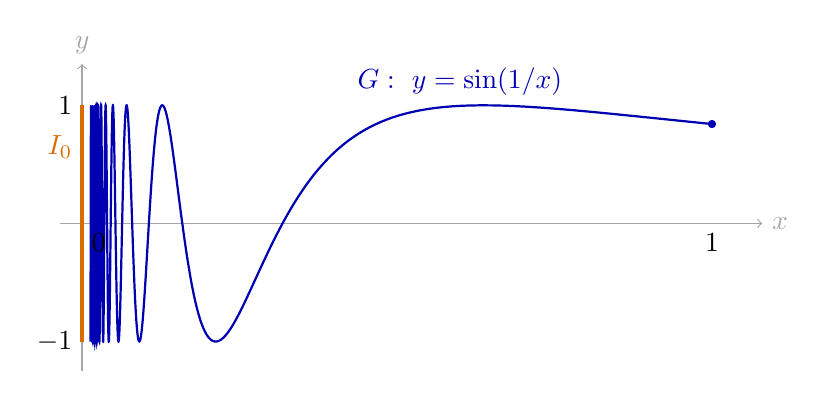
\begin{tikzpicture}[x=8cm,y=1.5cm]
	\draw[->,gray!70] (-0.035,0)--(1.08,0) node[right] {\(x\)};
	\draw[->,gray!70] (0,-1.25)--(0,1.35) node[above] {\(y\)};
	\draw[very thick,orange!85!black] (0,-1)--(0,1);
	\draw[blue!70!black,thick,domain=1:75,samples=1800,variable=\t] plot ({1/\t},{sin(\t r)});
	\fill[blue!70!black] (1,{sin(1 r)}) circle(1.5pt);
	\node[orange!85!black,left] at (0,0.65) {\(I_0\)};
	\node[blue!70!black] at (0.6,1.2) {\(G:\ y=\sin(1/x)\)};
	\node[below] at (1,0) {\(1\)};
	\node[left] at (0,-1) {\(-1\)};
	\node[left] at (0,1) {\(1\)};
	\node[below right] at (0,0) {\(0\)};
\end{tikzpicture}

	\caption[拓扑正弦曲线]{拓扑正弦曲线 \(S=G\cup I_0\)。曲线 \(G\) 不断靠近竖线段 \(I_0\)，使整个集合连通；沿一条道路离开竖线段却会迫使纵坐标在任意短的参数时间内反复走遍 \([-1,1]\)，与连续性矛盾。左侧密集振荡仅画出有限部分。}
	\label{g1:fig:topologist-sine}
\end{figure}

图中的竖线段不是与曲线“隔着一个正距离”的另一块：它的每个点都是曲线的极限点。这解释了为什么集合没有开集分离；道路的障碍则来自趋近竖线段时无限振荡的纵坐标。连通与道路连通分别检测了这两件不同的事。

\begin{definition}[局部道路连通]\label{g1:def:locally-path-connected}
	若拓扑空间 \(X\) 的每个点 \(x\)，在每个给定开邻域 \(U\) 中，都有一个道路连通开邻域 \(V\) 满足 \(x\in V\subseteq U\)，则称 \(X\)\term[jubudaoluliantong]{局部道路连通}[locally path-connected]。
\end{definition}

定义要求能够任意缩小，并非仅要求每点落在某个道路连通开集中。Euclid 开集局部道路连通，因为充分小的开球凸；局部同胚于 Euclid 开集的空间也局部道路连通，只需把小球送回原空间。拓扑正弦曲线在竖线段上的任何点都没有道路连通开邻域：每个这样的开邻域都遇到 \(G\)，而上一例已证明不存在从竖线段到 \(G\) 的道路。

\subsection{分支及其在映射下的行为}
\label{g1:subsec:0402:04}

一个空间未必整体连通，此时可以按“属于同一个连通部分”把点分组。这里的“部分”应是最大的连通子集，而不能只是任意选出的一个连通邻域；否则分组会依赖选择。

\begin{definition}[连通分支与道路分支]\label{g1:def:components}
	拓扑空间 \(X\) 的极大非空连通子集称为\term[liantongfenzhi]{连通分支}[connected component]。对 \(x\in X\)，所有可用道路从 \(x\) 到达的点组成的集合称为 \(x\) 的\term[daolufenzhi]{道路分支}[path component]。
\end{definition}

反向参数 \(t\mapsto1-t\) 可以反转道路；把两条道路分别重参数化到 \([0,1/2]\)、\([1/2,1]\) 并在公共端点相接，便可拼成一条道路。拼接的连续性由闭集粘合\cref{g1:prop:gluing-lemma}保证，因为两段在 \(t=1/2\) 取值相同。再加上常值道路，“可以用道路相连”就是等价关系。每个等价类本身道路连通：连接其中两点的道路经过的任一点，都能通过取道路的一段而与这两点相连，所以整条道路都留在同一个等价类中。因此道路分支也就是极大道路连通子集。

\begin{proposition}[分支的存在与基本性质]\label{g1:prop:components}
	设 \(X\) 为拓扑空间。
	\begin{enumerate}
		\item 对每个 \(x\in X\)，包含 \(x\) 的所有连通子集之并 \(C_x\) 是唯一包含 \(x\) 的连通分支；各连通分支构成 \(X\) 的一个划分。
		\item 每个连通分支闭于 \(X\)，但不一定开。每个道路分支包含在唯一的连通分支中。
		\item 若 \(f:X\to Y\) 连续，则一个连通分支的像包含在 \(Y\) 的某个连通分支中，一个道路分支的像包含在 \(Y\) 的某个道路分支中。
	\end{enumerate}
\end{proposition}
\begin{proof}
	第一项中，所有参加并集的连通子集都含 \(x\)，所以由\cref{g1:prop:connected-image-closure}，它们的并 \(C_x\) 连通。任何包含 \(x\) 的连通子集都已在此并中，因此 \(C_x\) 极大且唯一。如果两个这样的集合相交，它们的并仍连通，极大性便使两者相等；每个点至少属于自己的 \(C_x\)，所以这些分支构成划分。

	第二项中，\(\overline{C_x}\) 由同一命题仍连通，且包含 \(C_x\)，极大性给出 \(\overline{C_x}=C_x\)，故 \(C_x\) 闭。道路分支道路连通，因而连通，所以它包含在唯一的 \(C_x\) 中。连通分支未必开，例如 \(\mathbb Q\) 中每个连通分支都是单点，却没有单点是开集，证明见习题。

	第三项中，连通分支的连续像连通，因而被包含在其中任一点所属的连通分支中。对于道路分支，用道路与 \(f\) 复合即可说明其像道路连通，故同样被包含在某个道路分支中。
\end{proof}

此处结论是“包含在”，不能改成“等于”。例如常值映射把任意连通空间送到 \(\mathbb R\) 的一个点，而 \(\mathbb R\) 的连通分支是整个直线。甚至映射本身满射，也未必把每个分支满射到目标分支，习题将给出例子。

\begin{theorem}[局部道路连通时两种分支一致]\label{g1:thm:locally-path-components}
	若 \(X\) 局部道路连通，则 \(X\) 的每个道路分支都是开集，并且道路分支与连通分支相同。因此局部道路连通空间连通，当且仅当它道路连通。
\end{theorem}
\begin{proof}
	设 \(P\) 为一个道路分支，\(x\in P\)。局部道路连通性给出 \(x\) 的道路连通开邻域 \(V\)。\(V\) 中每点都能与 \(x\) 用道路连接，故 \(V\subseteq P\)。因此 \(P\) 中每点都有包含在 \(P\) 内的开邻域，\(P\) 开。

	设 \(C\) 为包含 \(P\) 的连通分支。若 \(C\setminus P\ne\varnothing\)，因为其他道路分支也开，\(X\setminus P\) 是开集；于是 \(P=C\cap P\) 与 \(C\setminus P=C\cap(X\setminus P)\) 是 \(C\) 的两个非空、不交相对开集，其并为 \(C\)，与 \(C\) 连通矛盾。因此 \(C=P\)。对非空连通空间，唯一的连通分支就是整个空间，所以结论随之成立；空空间也符合约定。
\end{proof}

拓扑正弦曲线说明局部条件的作用：它只有一个连通分支 \(S\)，却有两个道路分支 \(G,I_0\)，其中 \(I_0\) 不是开集。流形的局部 Euclid 性质则排除了这种现象。在流形上讨论某一连通分支时，也就在讨论一个开且道路连通的部分；这将允许我们把沿道路的局部构造在同一分支内传递。有关连通性、紧性和局部紧性的进一步阅读，可参阅\cite[第4章, Connectedness, 第86页; Compactness, 第94页; Local Compactness, 第104页]{Lee2011Topological}。

% !TeX root = ../../Book1.tex
% 纲要标题：### 4.3 流形所需的分离与可数性
% 纲要位置：几何学计划纲要.md，第 252 行。
% 正文状态：初稿；尚未正式审核。

% 纲要内容开始
% 
% * Hausdorff、正则与正规空间
% * 第二可数和可数穷竭
% * 局部紧、第二可数 Hausdorff 空间的仿紧性
% * Urysohn 引理与正则第二可数空间的度量化
% 
% 纲要内容结束

\section{流形所需的分离与可数性}
\label{g1:sec:0403}

Euclid 空间有两种看似不同的便利：可以把一个闭集与外面的点隔开，也可以用可数个小球描述所有开集。前一种便利允许我们在邻域内部留出余地，后一种便利使全空间上的选择能够按序组织。它们结合起来，将产生紧集穷竭、局部有限覆盖和与原拓扑相容的距离。本节把这些结论的假设逐项分开；后面定义流形时采用 Hausdorff 和第二可数条件，正是为了能够使用这些整体构造。

\subsection{Hausdorff、正则与正规空间}
\label{g1:subsec:0403:01}

\cref{g1:def:hausdorff}中的 Hausdorff 条件要求不同的两个点有不交开邻域。但在构造函数时，我们常要让一个函数在整块闭集上取零，而在另一块闭集上取一；只分离两个点还不够。下面的条件依次扩大需要分离的对象。

\begin{definition}[分离条件]\label{g1:def:regular-normal}
	设 \(X\) 为拓扑空间。若每个单点集都闭，称 \(X\) 满足\term[t1kongjian]{\(T_1\) 条件}[\(T_1\) separation axiom]。本书采用以下约定。
	\begin{enumerate}
		\item 若 \(X\) 满足 \(T_1\) 条件，且对每个闭集 \(F\subseteq X\) 及每个 \(x\notin F\)，都存在不交开集 \(U,V\)，使 \(x\in U\)、\(F\subseteq V\)，则称它为\term[zhengzekongjian]{正则空间}[regular space]。
		\item 若 \(X\) 满足 \(T_1\) 条件，且任意两个不交闭集 \(A,B\subseteq X\) 都有不交开邻域，则称它为\term[zhengguikongjian]{正规空间}[normal space]。
	\end{enumerate}
\end{definition}

一些文献把上述分离性质与 \(T_1\) 条件分开命名，因此使用外部结果时需要核对约定。在本书的约定下，
\[
	\text{正规}\ \Longrightarrow\ \text{正则}\ \Longrightarrow\ \text{Hausdorff}\ \Longrightarrow\ T_1.
\]
前两个箭头分别把一个闭集取成单点、把两个闭集都取成单点。最后一个箭头来自：若 \(y\ne x\)，Hausdorff 条件给出一个含 \(y\) 而不含 \(x\) 的开邻域；这些邻域之并是 \(X\setminus\{x\}\)。

\begin{lemma}[分离与邻域缩小]\label{g1:lem:regular-normal-shrink}
	设 \(X\) 满足 \(T_1\) 条件。
	\begin{enumerate}
		\item \(X\) 正则，当且仅当对每个 \(x\in G\)（\(G\) 开），存在开集 \(V\)，使 \(x\in V\subseteq\overline V\subseteq G\)。
		\item \(X\) 正规，当且仅当对每个闭集 \(A\) 和包含它的开集 \(G\)，存在开集 \(V\)，使 \(A\subseteq V\subseteq\overline V\subseteq G\)。
	\end{enumerate}
\end{lemma}
\begin{proof}
	先看第二项。若 \(X\) 正规，对不交闭集 \(A\) 与 \(X\setminus G\) 取不交开邻域 \(V,W\)。因为 \(X\setminus W\) 闭且包含 \(V\)，有 \(\overline V\subseteq X\setminus W\subseteq G\)。反之，对不交闭集 \(A,B\)，把缩小性质用于 \(A\subseteq X\setminus B\)。所得 \(V\) 与 \(X\setminus\overline V\) 是分别包含 \(A,B\) 的不交开集。第一项的论证相同，只需把 \(A\) 换成单点 \(\{x\}\)。
\end{proof}

把闭包也留在原邻域内的缩小方式，为取极限、控制支集与零延拓留出了余地。\cref{g1:lem:local-compact-shrink}已经说明，局部紧 Hausdorff 空间具有这种点的邻域缩小性质，而且可以要求闭包紧。因此局部紧 Hausdorff 空间正则；此处尚未要求它第二可数。

\begin{example}[度量空间中的分离函数]\label{g1:exm:metric-normal}
	每个度量空间 \((X,d)\) 都正规。单点集闭；若 \(A,B\) 是非空不交闭集，令
	\[
		d(x,A)=\inf_{a\in A}d(x,a),\qquad
		h(x)=\frac{d(x,A)}{d(x,A)+d(x,B)}.
	\]
	三角不等式给出 \(|d(x,A)-d(y,A)|\le d(x,y)\)，故两个距离函数连续。又因 \(A,B\) 闭且不交，它们的距离函数不可能在同一点同时为零，所以分母处处为正。于是 \(h\) 连续，在 \(A\) 上为零，在 \(B\) 上为一；开集 \(\{h<1/3\}\) 与 \(\{h>2/3\}\) 分离 \(A,B\)。若有一个闭集为空，直接取空集和全空间即可。
\end{example}

这里没有要求两个闭集之间的距离为正。例如平面中 \(A=\{(t,0):t\ge1\}\) 与 \(B=\{(t,1/t):t\ge1\}\) 都闭，二者距离的下确界却为零。上例只需要每个固定点处的分母为正，并不需要全空间上一致的正下界。

\subsection{第二可数和可数穷竭}
\label{g1:subsec:0403:02}

为了在不同地方选择局部数据，我们希望这些选择能够列成一张可数清单。局部与整体的可数性具有不同的量词：“每一点有可数个基本邻域”允许不同的点各自使用一张清单；“全空间有可数个基本开集”要求一张清单适用于所有点。

\begin{definition}[可数性条件]\label{g1:def:countability}
	设 \(X\) 为拓扑空间。若每一点 \(x\) 都有可数邻域基，即存在含 \(x\) 的开集 \(U_1,U_2,\ldots\)，使每个含 \(x\) 的开集都包含某个 \(U_n\)，则称该空间\term[diyikeshu]{第一可数}[first countable]。若 \(X\) 的整个拓扑有一个可数基，则称它\term[dierkeshu]{第二可数}[second countable]。若 \(X\) 有可数稠密子集，称它\term[kefenkongjian]{可分}[separable]。若每个开覆盖都有可数子覆盖，称它具有\term[lindelofxingzhi]{Lindelöf 性质}[Lindelöf property]。\footnote{Ernst Leonard Lindelöf（1870--1946），芬兰数学家，研究函数论与微分方程。}
\end{definition}

可数在这里包括有限。第二可数立即蕴含第一可数：只取全空间的基中那些包含给定点的成员。每个度量空间都第一可数，因为 \(B(x,1/n)\) 构成 \(x\) 的邻域基；但一个度量空间不一定第二可数。若一个离散空间不可数，其每个单点都是开集，任何拓扑基都必须包含所有单点。

\begin{proposition}[第二可数的两项后果]\label{g1:prop:second-countable-lindelof}
	第二可数空间是可分空间，并具有 Lindelöf 性质。第二可数性遗传给任意子空间；Lindelöf 性质遗传给闭子空间。
\end{proposition}
\begin{proof}
	设 \(\{B_n\}\) 是可数基，忽略空的基元素。在每个 \(B_n\) 中取一点 \(x_n\)，所得可数点集与每个非空开集相交，因为每个这样的开集都包含某个 \(B_n\)。所以它稠密。

	给定开覆盖 \(\mathcal U\)，对每个能够包含在某个覆盖成员中的 \(B_n\)，选定一个这样的 \(U_n\in\mathcal U\)。所得至多可数个 \(U_n\) 覆盖 \(X\)：若 \(x\in U\in\mathcal U\)，基的性质给出 \(x\in B_n\subseteq U\)，于是选定的 \(U_n\) 也包含 \(x\)。

	若 \(Y\subseteq X\)，则 \(\{B_n\cap Y\}\) 是子空间的可数基。最后设 \(F\) 是 Lindelöf 空间 \(X\) 的闭子集，且 \(\{F\cap U_\alpha\}\) 是 \(F\) 的相对开覆盖，其中 \(U_\alpha\) 在 \(X\) 中开。把 \(X\setminus F\) 加入 \(\{U_\alpha\}\) 得到 \(X\) 的开覆盖，取可数子覆盖再与 \(F\) 相交即可。
\end{proof}

在 Euclid 空间中，以有理坐标点为中心、正有理数为半径的开球构成可数基。其关键不只是中心稠密，还在于可以把半径取得足够小：给定 \(x\in U\)，先取 \(B(x,\varepsilon)\subseteq U\)，再取靠近 \(x\) 的有理点 \(q\) 和满足 \(\lVert x-q\rVert<r<\varepsilon-\lVert x-q\rVert\) 的正有理数 \(r\)，便有 \(x\in B(q,r)\subseteq U\)。

\begin{definition}[紧穷竭]\label{g1:def:compact-exhaustion}
	设 \(X\) 为拓扑空间。一列紧集 \((K_n)_{n\ge1}\) 若满足
	\[
		K_n\subseteq\operatorname{int}K_{n+1},\qquad
		X=\bigcup_{n\ge1}K_n,
	\]
	称为 \(X\) 的一个\term[jinqiongjie]{紧穷竭}[compact exhaustion]。内部和闭包均在 \(X\) 中计算。
\end{definition}

\cref{g1:def:locally-compact}中的相对紧是指子集在环境空间中的闭包紧。下面会先得到由相对紧开集组成的可数基，再把这些开集分批装进紧穷竭。

\begin{theorem}[可数相对紧基与紧穷竭]\label{g1:thm:compact-exhaustion}
	局部紧、第二可数的 Hausdorff 空间 \(X\) 有可数相对紧开基，并有紧穷竭。对这样的穷竭，每个紧子集 \(C\subseteq X\) 都包含于某个 \(\operatorname{int}K_N\)。
\end{theorem}
\begin{proof}
	空空间取所有 \(K_n=\varnothing\)。以下设 \(X\ne\varnothing\)。从一个可数开基出发，只保留相对紧的基元素。它们仍是基：给定 \(x\in U\) 且 \(U\) 开，\cref{g1:lem:local-compact-shrink}给出开集 \(V\)，满足 \(x\in V\)、\(\overline V\) 紧且 \(\overline V\subseteq U\)。再选原来的基元素 \(B\) 使 \(x\in B\subseteq V\)，则 \(\overline B\) 是紧集 \(\overline V\) 的闭子集，因而紧。这里闭包包含于 \(\overline V\) 的事实也保证了 \(B\subseteq U\)。

	把保留下来的非空基元素列成 \(B_1,B_2,\ldots\)；若只有有限个，可以重复列出。令 \(K_1=\overline B_1\)。已构造 \(K_n\) 后，紧集 \(K_n\cup\overline B_{n+1}\) 可由有限个基元素 \(B_{j_1},\ldots,B_{j_s}\) 覆盖。定义
	\[
		K_{n+1}=\overline B_{j_1}\cup\cdots\cup\overline B_{j_s}.
	\]
	这是有限个紧集之并，仍紧，而且
	\[
		K_n\cup\overline B_{n+1}
		\subseteq B_{j_1}\cup\cdots\cup B_{j_s}
		\subseteq\operatorname{int}K_{n+1}.
	\]
	因此所需的内部包含关系成立，各 \(B_n\) 也都被某个 \(K_n\) 包含，故这些紧集穷尽 \(X\)。

	最后，由 \(K_n\subseteq\operatorname{int}K_{n+1}\)，开集 \(\operatorname{int}K_n\) 覆盖 \(X\)。它们递增，所以对紧集 \(C\) 取有限子覆盖后，最大的下标 \(N\) 已满足 \(C\subseteq\operatorname{int}K_N\)。
\end{proof}

紧穷竭除了满足 \(X=\bigcup_nK_n\)，还通过相邻紧集的内部包含关系留出余地。内部包含关系使 \(K_n\) 与 \(X\setminus K_{n+1}\) 之间隔着一层开邻域；下一小节将利用这层余地，让越来越远处选择的开集不再影响一个固定点附近。

\subsection{局部紧、第二可数 Hausdorff 空间的仿紧性}
\label{g1:subsec:0403:03}

在一个非紧空间上，开覆盖通常不能缩减为有限覆盖。然而粘合函数时，全空间上只有有限项并非必需：只要每个点附近实际上只有有限项出现，求和的连续性便仍是有限和的连续性。这就是局部有限条件的作用。

\begin{definition}[细化、局部有限与仿紧]\label{g1:def:locally-finite-refinement}
	设 \(\mathcal U\) 是 \(X\) 的覆盖，\(\mathcal V\) 是另一个覆盖。若每个 \(V\in\mathcal V\) 都包含于某个 \(U\in\mathcal U\)，则称新覆盖为原覆盖的\term[xihua]{细化}[refinement]。对于一族子集 \(\{A_i\}_{i\in I}\)，若每个 \(x\in X\) 都有一个只与有限个 \(A_i\) 相交的开邻域，则称这族集合是\term[jubuyouxian]{局部有限}[locally finite]的。若 \(X\) 的每个开覆盖都有局部有限开细化，称 \(X\) 为\term[fangjinkongjian]{仿紧空间}[paracompact space]。本书的仿紧性定义本身不包含 Hausdorff 条件。
\end{definition}

细化可以增加覆盖成员的数目；它要求新开集更贴合原覆盖，并不要求新覆盖是原覆盖的子族。局部有限也不同于“每个点只属于有限个成员”：后一条件只控制点本身，前一条件还控制它附近的所有点。例如 \(\{(1/(n+1),1/n):n\ge1\}\) 在 \(\mathbb R\) 中每点至多属于一个成员，却在 \(0\) 附近不是局部有限的。

\begin{lemma}[局部有限与闭包]\label{g1:lem:locally-finite-closures}
	若 \(\{A_i\}_{i\in I}\) 是拓扑空间 \(X\) 中的局部有限族，则 \(\{\overline A_i\}_{i\in I}\) 仍局部有限，并且
	\[
		\overline{\bigcup_{i\in I}A_i}=\bigcup_{i\in I}\overline A_i.
	\]
	特别地，局部有限闭集族的并是闭集；其任意子族的并也闭。
\end{lemma}
\begin{proof}
	若开集 \(N\) 与 \(\overline A_i\) 相交，取交点后利用闭包定义可知 \(N\) 也与 \(A_i\) 相交。因此一个只与有限个 \(A_i\) 相交的开邻域，也只与对应的有限个闭包相交。

	为证明右边的并闭，取 \(x\notin\bigcup_i\overline A_i\)，并取只与有限个闭包 \(\overline A_{i_1},\ldots,\overline A_{i_s}\) 相交的开邻域 \(N\)。开集 \(N\setminus\bigcup_{k=1}^s\overline A_{i_k}\) 包含 \(x\)，且与所有闭包都不交。故右边是包含 \(\bigcup_iA_i\) 的闭集，包含其闭包。反向包含逐项由 \(A_i\subseteq\bigcup_jA_j\) 得到。子族仍局部有限，最后一句随即成立。
\end{proof}

\begin{theorem}[由紧穷竭得到局部有限细化]\label{g1:thm:lch-paracompact}
	设 \(X\) 为局部紧、第二可数的 Hausdorff 空间。对 \(X\) 的每个开覆盖 \(\mathcal U\)，存在可数的局部有限开覆盖 \(\{V_j\}\)，使每个 \(\overline V_j\) 都紧，并包含于某个 \(U\in\mathcal U\)。特别地，\(X\) 仿紧。
\end{theorem}
\begin{proof}
	由\cref{g1:thm:compact-exhaustion}取紧穷竭 \((K_n)\)，并约定 \(K_{-1}=K_0=\varnothing\)。把 \(X\) 分成相互允许重叠的紧壳层
	\[
		S_n=K_n\setminus\operatorname{int}K_{n-1},
		\qquad
		G_n=\operatorname{int}K_{n+1}\setminus K_{n-2}.
	\]
	每个 \(S_n\) 紧，每个 \(G_n\) 开，而且 \(S_n\subseteq G_n\)：外侧包含来自 \(K_n\subseteq\operatorname{int}K_{n+1}\)，内侧避开 \(K_{n-2}\) 则来自 \(K_{n-2}\subseteq\operatorname{int}K_{n-1}\)。这些 \(S_n\) 覆盖 \(X\)，因为每个点第一次进入某个 \(K_n\) 时就属于 \(S_n\)。

	对每个 \(x\in S_n\)，选原覆盖成员 \(U_x\) 包含 \(x\)，再由\cref{g1:lem:local-compact-shrink}在开集 \(G_n\cap U_x\) 中缩小邻域，得到
	\[
		x\in V_x,\qquad
		\overline V_x\text{ 紧},\qquad
		\overline V_x\subseteq G_n\cap U_x.
	\]
	利用 \(S_n\) 紧，为这一层保留有限个 \(V_{n,1},\ldots,V_{n,r_n}\)。空壳层不需选择成员。所有层的选择合起来是可数开细化，并覆盖 \(X\)。

	剩下要证明的是局部有限；每层有限还不足以直接给出这个结论。给定 \(x\in X\)，选 \(m\) 使 \(x\in\operatorname{int}K_m\)。当 \(n\ge m+2\) 时，\(K_m\subseteq K_{n-2}\)，而这一层的全部 \(V_{n,k}\) 都位于 \(G_n\subseteq X\setminus K_{n-2}\)，故它们与 \(\operatorname{int}K_m\) 不交。于是该邻域只可能遇到前 \(m+1\) 层中的有限个成员，这正是局部有限。
\end{proof}

在这个构造中，\(S_n\) 是需要覆盖的区域，\(G_n\) 是允许选择邻域的稍大区域。让第 \(n\) 层避开 \(K_{n-2}\)，而不只要求它留在 \(K_{n+1}\) 以内，保证了远处的开集不会重新伸回固定点附近。

\begin{figure}[htbp]
	\centering
	% !TeX root = ../Book1.tex
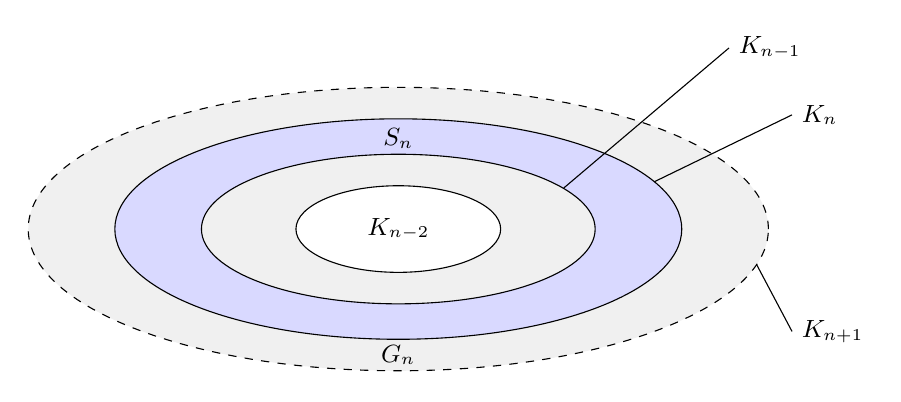
\begin{tikzpicture}[x=1cm,y=1cm,font=\small]
	\fill[gray!12,even odd rule] (0,0) ellipse (4.7 and 1.8) (0,0) ellipse (1.3 and .55);
	\fill[blue!15,even odd rule] (0,0) ellipse (3.6 and 1.4) (0,0) ellipse (2.5 and .95);
	\draw[dashed] (0,0) ellipse (4.7 and 1.8);
	\draw (0,0) ellipse (3.6 and 1.4);
	\draw (0,0) ellipse (2.5 and .95);
	\draw (0,0) ellipse (1.3 and .55);
	\node at (0,0) {\(K_{n-2}\)};
	\node at (0,1.15) {\(S_n\)};
	\node at (0,-1.6) {\(G_n\)};
	\draw (2.1,.52) -- (4.2,2.3) node[right] {\(K_{n-1}\)};
	\draw (3.25,.6) -- (5,1.45) node[right] {\(K_n\)};
	\draw (4.55,-.45) -- (5,-1.3) node[right] {\(K_{n+1}\)};
\end{tikzpicture}

	\caption{蓝色壳层 \(S_n\) 位于灰色区域 \(G_n\) 内，内外各留一层余地。曲线仅表示包含关系，并未假定空间嵌入平面。}
	\label{g1:fig:compact-exhaustion-shells}
\end{figure}

\begin{theorem}[仿紧 Hausdorff 空间的正规性]\label{g1:thm:paracompact-normal}
	每个仿紧 Hausdorff 空间都是正规空间。
\end{theorem}
\begin{proof}
	先证明正则性，不能在这一步预先使用闭包缩小。给定闭集 \(F\) 和 \(x\notin F\)，对每个 \(y\in F\)，由 Hausdorff 条件取分别含 \(x,y\) 的不交开集 \(P_y,Q_y\)。于是 \(x\notin\overline{Q_y}\)。对开覆盖
	\[
		\{X\setminus F\}\cup\{Q_y:y\in F\}
	\]
	取局部有限开细化 \(\{W_i\}_{i\in I}\)，并令 \(I_F=\{i:W_i\cap F\ne\varnothing\}\)。若 \(i\in I_F\)，则 \(W_i\) 不可能包含于 \(X\setminus F\)，所以必包含于某个 \(Q_y\)，从而 \(x\notin\overline W_i\)。由\cref{g1:lem:locally-finite-closures}，
	\[
		H=\bigcup_{i\in I_F}\overline W_i
	\]
	是一个不含 \(x\) 的闭集。于是 \(X\setminus H\) 与 \(\bigcup_{i\in I_F}W_i\) 是分别包含 \(x,F\) 的不交开集。Hausdorff 条件已保证 \(T_1\)，故 \(X\) 正则。

	现在设 \(A,B\) 是不交闭集。由刚证的正则性及\cref{g1:lem:regular-normal-shrink}，对每个 \(a\in A\) 取开集 \(O_a\)，满足 \(a\in O_a\)、\(\overline O_a\subseteq X\setminus B\)。对覆盖
	\[
		\{X\setminus A\}\cup\{O_a:a\in A\}
	\]
	再取局部有限开细化 \(\{V_j\}_{j\in J}\)。保留那些与 \(A\) 相交的成员，其下标集记为 \(J_A\)。每个这样的 \(V_j\) 必包含于某个 \(O_a\)，所以它的闭包避开 \(B\)。局部有限性保证 \(F_A=\bigcup_{j\in J_A}\overline V_j\) 闭，且仍避开 \(B\)。因此 \(\bigcup_{j\in J_A}V_j\) 与 \(X\setminus F_A\) 是 \(A,B\) 的不交开邻域，得到正规性。
\end{proof}

紧空间的每个开覆盖都有有限子覆盖，而有限族总是局部有限的。因此紧 Hausdorff 空间正规；这里紧性提供有限子覆盖，Hausdorff 条件负责最初的点分离。对流形将使用的局部紧、第二可数 Hausdorff 空间，上面两条定理则把“局部紧”转化成了整个空间上的正规性。

\subsection{Urysohn 引理与正则第二可数空间的度量化}
\label{g1:subsec:0403:04}

如果拓扑已经来自距离，\cref{g1:exm:metric-normal}用距离函数构造了取值在 \([0,1]\) 中的连续分离函数。现在反过来：先仅用开集与闭集构造足够多的这样的函数，再把函数值的差组合成距离。需要解决两个问题：如何在没有距离时构造连续函数，以及如何把全空间的分离任务缩减到可数个函数。

\begin{lemma}[正则 Lindelöf 空间的正规性]\label{g1:lem:regular-lindelof-normal}
	每个正则且具有 Lindelöf 性质的空间都是正规空间。
\end{lemma}
\begin{proof}
	设 \(A,B\) 为不交闭集。由正则性，为 \(A\) 的各点取闭包避开 \(B\) 的开邻域。闭子空间 \(A\) 仍有 Lindelöf 性质，故可取可数个这样的开集 \(U_n\) 覆盖 \(A\)。同样可取开集 \(V_n\) 覆盖 \(B\)，使 \(\overline V_n\cap A=\varnothing\)。若某一族有限或为空，可补空集写成数列。令
	\[
		U=\bigcup_{n\ge1}\left(U_n\setminus\bigcup_{i=1}^n\overline V_i\right),
		\qquad
		V=\bigcup_{n\ge1}\left(V_n\setminus\bigcup_{i=1}^n\overline U_i\right).
	\]
	括号中只减去有限个闭集，因而 \(U,V\) 都开。因为所有 \(\overline V_i\) 避开 \(A\)，\(U\) 仍包含 \(A\)；同理 \(V\) 包含 \(B\)。若某点同时落在左边第 \(n\) 项与右边第 \(m\) 项中，当 \(m\le n\) 时，左边已减去 \(\overline V_m\)，不可能属于 \(V_m\)；当 \(n\le m\) 时，右边已减去 \(\overline U_n\)，同样矛盾。因此 \(U\cap V=\varnothing\)。
\end{proof}

这个交错删去有限个闭集的构造解释了可数性的用途：第 \(n\) 个开集只需避开对方的前 \(n\) 个闭包，而任意一对下标终究有一个先后关系。若直接从每个 \(U_n\) 中减去对方所有闭包，剩下的集合未必开。

\begin{lemma}[Urysohn 引理]\label{g1:lem:urysohn}
	设 \(X\) 为正规空间，\(A,B\subseteq X\) 为不交闭集。则存在连续函数 \(f:X\to[0,1]\)，使 \(f|_A=0\)、\(f|_B=1\)。
\end{lemma}

这一结果称为\term[urysohnyinli]{Urysohn 引理}[Urysohn lemma]。\footnote{Pavel Samuilovich Urysohn（1898--1924），苏联数学家，研究一般拓扑与维数理论。}构造从安排函数的“低于某一高度的区域”入手。为保证函数连续，不同高度之间需要留出闭包包含关系。

\begin{proof}
	令 \(D=\{k/2^m:0\le k\le2^m,\ m\ge0\}\subseteq[0,1]\) 为二进有理数集。我们要为每个 \(r\in D\) 构造开集 \(U_r\)，使
	\[
		A\subseteq U_0,\qquad U_1=X\setminus B,\qquad
		\overline U_r\subseteq U_s\quad(r<s,\ r,s\in D).
	\]
	先由\cref{g1:lem:regular-normal-shrink}，为闭集 \(A\subseteq X\setminus B\) 取开邻域 \(U_0\)，满足 \(\overline U_0\subseteq U_1=X\setminus B\)。假设分母为 \(2^m\) 的各开集已经构造。对相邻的 \(r=k/2^m\) 与 \(s=(k+1)/2^m\)，在闭集 \(\overline U_r\subseteq U_s\) 之间再缩小一次，得到
	\[
		\overline U_r\subseteq U_{(r+s)/2}
		\subseteq\overline U_{(r+s)/2}\subseteq U_s.
	\]
	每一层只加入这些中间开集，旧的开集保持不变。任意两个二进有理数都出现在某个共同的有限层中，逐个使用相邻包含关系，便得到全部所需的嵌套关系。

	定义
	\[
		f(x)=\inf\bigl(\{r\in D:x\in U_r\}\cup\{1\}\bigr).
	\]
	加入 \(\{1\}\) 使这个集合总非空，所以 \(f\) 在每一点都有定义并属于 \([0,1]\)。若 \(x\in A\)，则 \(x\in U_0\)，故 \(f(x)=0\)；若 \(x\in B\)，则它不属于任何 \(U_r\)，故 \(f(x)=1\)。

	下面分别检验函数值低于和高于给定高度的集合开。对 \(0<a\le1\)，下确界的性质给出
	\[
		\{f<a\}=\bigcup_{\substack{r\in D\\r<a}}U_r.
	\]
	对 \(0\le a<1\)，则有
	\[
		\{f>a\}=\bigcup_{\substack{r\in D\\a<r<1}}(X\setminus\overline U_r).
	\]
	为核对第二式，若 \(x\notin\overline U_r\)，则它不属于任何 \(U_t\)（\(t<r\)），所以 \(f(x)\ge r>a\)。反之，若 \(f(x)>a\)，取二进有理数 \(a<r<f(x)\)。若 \(x\in\overline U_r\)，则对每个二进有理数 \(s>r\) 都有 \(x\in U_s\)，从而 \(f(x)\le r\)，矛盾。故 \(x\notin\overline U_r\)。这证明第二式。上述两个集合都开；当 \(a\) 在其余范围时，它们是空集或全空间。实数开区间的原像由这两类集合相交得到，故 \(f\) 连续。
\end{proof}

若映射 \(F:X\to Y\) 是 \(X\) 到其像 \(F(X)\) 的同胚，其中像赋予 \(Y\) 的子空间拓扑，就称 \(F\) 为\term[tuopuqianru]{拓扑嵌入}[topological embedding]。下面将用可数个连续函数把原空间实现为一个可数积空间的子空间。

\begin{theorem}[Urysohn 度量化定理]\label{g1:thm:urysohn-metrization}
	设 \(X\) 为正则、第二可数的拓扑空间。则存在一列连续函数 \(f_n:X\to[0,1]\)，使
	\begin{equation}\label{g1:eq:urysohn-metric}
		d(x,y)=\sum_{n=1}^{\infty}2^{-n}|f_n(x)-f_n(y)|
	\end{equation}
	成为 \(X\) 上的度量，并且它所诱导的拓扑恰好等于原拓扑。映射 \(x\mapsto(f_n(x))_{n\ge1}\) 将 \(X\) 拓扑嵌入带积拓扑的 \([0,1]^{\mathbb N}\)。
\end{theorem}

若一个空间的拓扑可由某个距离诱导，就称这个空间\term[kelianghua]{可度量化}[metrizable]；并不预先指定距离，也不保证这个距离完备。上述结果称为\term[urysohndulianghua]{Urysohn 度量化定理}[Urysohn metrization theorem]。这里正则性含 \(T_1\) 条件。定理比“局部紧、第二可数 Hausdorff 空间可度量化”更一般，因为它不要求局部紧。

\begin{proof}
	空空间的结论按空映射成立。设 \(X\ne\varnothing\)，取可数开基 \(\{B_i\}\)。由\cref{g1:prop:second-countable-lindelof,g1:lem:regular-lindelof-normal}，\(X\) 正规。对每一对满足 \(\overline B_i\subseteq B_j\) 的下标 \((i,j)\)，把\cref{g1:lem:urysohn}用于不交闭集 \(X\setminus B_j\) 与 \(\overline B_i\)，得到连续函数 \(f_{ij}:X\to[0,1]\)，满足
	\[
		f_{ij}=1\text{ 于 }\overline B_i,\qquad
		f_{ij}=0\text{ 于 }X\setminus B_j.
	\]
	这些下标对至多可数。列出全部所得函数，并在必要时补上常值零函数，记成 \((f_n)_{n\ge1}\)。

	这些函数具有比“分开两个点”更强的性质：若 \(x\in O\) 且 \(O\) 开，可以找到一个 \(f_k\)，使 \(f_k(x)=1\)，并在 \(X\setminus O\) 上为零。事实上，先取基元素 \(x\in B_j\subseteq O\)，再由正则性选 \(x\in V\subseteq\overline V\subseteq B_j\)，最后取 \(x\in B_i\subseteq V\)。于是 \(\overline B_i\subseteq B_j\)，所对应的 \(f_{ij}\) 就满足要求。特别地，对 \(x\ne y\)，因 \(T_1\) 条件使 \(X\setminus\{y\}\) 开，这一性质给出某个 \(f_k(x)=1\)、\(f_k(y)=0\)。

	现在用\eqref{g1:eq:urysohn-metric}定义 \(d\)。每项不超过 \(2^{-n}\)，故级数收敛。对称性与非负性逐项成立；刚证的点分离性质保证 \(x\ne y\) 时 \(d(x,y)>0\)。每个函数值差满足实数的三角不等式，把前 \(N\) 项相加再令 \(N\to\infty\)，得到 \(d(x,z)\le d(x,y)+d(y,z)\)。所以 \(d\) 是度量。

	还必须证明原来的开集与度量开集相同，单有点分离并不能保证这一点。给定 \(x\in X\) 与 \(\varepsilon>0\)，取 \(N\) 使 \(\sum_{n>N}2^{-n}<\varepsilon/2\)。由前 \(N\) 个函数的连续性，存在原拓扑中的开邻域 \(V\ni x\)，使对 \(y\in V\) 及 \(1\le n\le N\)，都有 \(|f_n(x)-f_n(y)|<\varepsilon/2\)。于是前 \(N\) 项之和小于 \(\varepsilon/2\)，尾项之和也小于 \(\varepsilon/2\)，故 \(V\subseteq B_d(x,\varepsilon)\)。这说明从原拓扑到度量拓扑的恒等映射连续。

	反过来，给定原拓扑的开邻域 \(O\ni x\)，取上述满足 \(f_k(x)=1\) 且在 \(X\setminus O\) 上为零的函数。如果 \(d(x,y)<2^{-k-1}\)，则
	\[
		2^{-k}|f_k(x)-f_k(y)|\le d(x,y)<2^{-k-1},
	\]
	所以 \(f_k(y)>1/2\)，从而 \(y\in O\)。因此 \(B_d(x,2^{-k-1})\subseteq O\)，另一方向的恒等映射也连续。

	最后，令 \(F(x)=(f_n(x))\)。它由点分离性质单射，而在立方体 \([0,1]^{\mathbb N}\) 上，
	\[
		D(s,t)=\sum_{n\ge1}2^{-n}|s_n-t_n|
	\]
	是一个度量，且 \(D(F(x),F(y))=d(x,y)\)。这个度量给出积拓扑：其开球包含由有限个坐标的小变化所确定的基本开邻域，理由正是上面的尾项估计；反过来，对规定有限个坐标的邻域，取球半径小于各坐标容许变化量乘以对应 \(2^{-n}\) 的最小值，整个球便包含于该邻域。因此 \(F\) 是 \(X\) 到其像的同胚，即所称的拓扑嵌入。
\end{proof}

可以把 \((f_n(x))\) 看作一列连续测量值。正则性与 Urysohn 引理保证：无论给点 \(x\) 指定多小的开邻域，总有一项测量在 \(x\) 取一、在邻域外取零。第二可数性把所有这种局部区分压缩为可数个测量；权重 \(2^{-n}\) 则让后面无穷多项的总影响可以统一控制。

\begin{corollary}[流形所用的拓扑结论]\label{g1:cor:lch-second-countable}
	每个局部紧、第二可数的 Hausdorff 空间都可度量化、仿紧且正规，并具有紧穷竭。
\end{corollary}
\begin{proof}
	局部紧 Hausdorff 空间由邻域缩小性质正则，因此可应用\cref{g1:thm:urysohn-metrization}。紧穷竭、仿紧性与正规性分别由\cref{g1:thm:compact-exhaustion,g1:thm:lch-paracompact,g1:thm:paracompact-normal}得到。
\end{proof}

这个推论给出与开集相容的点间距离，式\eqref{g1:eq:urysohn-metric}中的距离未必完备。Riemann 度量则在每个切空间上指定随点光滑变化的内积；下一节的连续单位分解将先说明这类局部数据怎样加权粘合。

% !TeX root = ../../Book1.tex
% 纲要标题：### 4.4 局部有限覆盖与单位分解
% 纲要位置：几何学计划纲要.md，第 259 行。
% 正文状态：初稿；尚未正式审核。

% 纲要内容开始
% 
% * 覆盖的细化与闭集收缩
% * 连续截断函数的构造
% * 从局部有限覆盖构造单位分解
% * 连续函数与正定双线性型的整体粘合
% 
% 纲要内容结束

\section{局部有限覆盖与单位分解}
\label{g1:sec:0404}

在一条直线的左侧使用一种公式、右侧使用另一种公式，如果两式在交叠处相同，就可以直接粘合。若它们各有用途，却不完全相同，又怎样平稳地过渡？一个自然想法是给两式分配非负权重，并使权重之和为 \(1\)。对于许多张局部坐标图，同样的想法要求我们同时解决三个问题：每个权重只在允许的区域起作用，各点附近只出现有限项，而且任一点至少有一个权重为正。本节用覆盖的收缩与连续截断函数逐项实现这些要求。

\subsection{覆盖的细化与闭集收缩}
\label{g1:subsec:0404:01}

\cref{g1:def:locally-finite-refinement}中的局部有限性说，每一点都有一个邻域，只与给定族中的有限多个集合相交。它比“每个点只属于有限多个集合”更强：前者控制了点附近的变化，后者只控制某一点上的计数。在 \(\mathbb R\) 中，令 \(c_n=2^{-n}\)、\(r_n=2^{-n-2}\)，闭区间 \([c_n-r_n,c_n+r_n]\) 两两不交，故每点至多属于一个，但原点的每个邻域都遇到无穷多个。这种聚集会使看似逐点有意义的和失去连续性。

已由\cref{g1:lem:locally-finite-closures}证明，局部有限族取闭包后仍局部有限，且局部有限闭集族的并为闭集。这里闭包结论中的“邻域”尤其有用：一个开集若不交某集合，也不交它的闭包。这使我们可以在同一个邻域内同时控制函数的非零区域与这些区域的边界。

\begin{lemma}[带闭包控制的细化与收缩]\label{g1:lem:cover-shrinking}
	设 \(X\) 为仿紧 Hausdorff 空间。
	\begin{enumerate}
		\item 对任意开覆盖 \(\{U_\alpha\}_{\alpha\in A}\)，存在局部有限开覆盖 \(\{V_j\}_{j\in J}\) 及指标选择 \(\alpha(j)\)，使 \(\overline{V_j}\subseteq U_{\alpha(j)}\)。
		\item 对任意局部有限开覆盖 \(\{V_j\}_{j\in J}\)，存在同指标闭集族 \(\{F_j\}_{j\in J}\)，满足 \(F_j\subseteq V_j\)、\(\bigcup_jF_j=X\)。这族闭集仍局部有限，允许某些 \(F_j\) 为空。
	\end{enumerate}
\end{lemma}
\begin{proof}
	由\cref{g1:thm:paracompact-normal}，\(X\) 正规，因而也正则。对每个 \(x\in X\)，先选包含它的一个 \(U_{\alpha_x}\)，再用正则性选开邻域 \(W_x\)，使
	\[
		x\in W_x\subseteq\overline{W_x}\subseteq U_{\alpha_x}.
	\]
	仿紧性给出开覆盖 \(\{W_x\}\) 的一个局部有限开细化 \(\{V_j\}\)。对每个 \(j\) 选 \(x(j)\) 使 \(V_j\subseteq W_{x(j)}\)，便有 \(\overline{V_j}\subseteq\overline{W_{x(j)}}\subseteq U_{\alpha_{x(j)}}\)，证明第一项。

	现从第二项给定的局部有限开覆盖 \(\{V_j\}\) 出发，把第一项用于它，得到局部有限开覆盖 \(\{W_k\}_{k\in K}\)，并为每个 \(k\) 选 \(j(k)\)，使 \(\overline{W_k}\subseteq V_{j(k)}\)。按被分配到的原指标合并，令
	\[
		F_j=\bigcup_{k:\,j(k)=j}\overline{W_k}.
	\]
	闭包族局部有限，故其中任何子族的并都闭；于是每个 \(F_j\) 是闭集，且 \(F_j\subseteq V_j\)。因为 \(W_k\) 覆盖 \(X\)，这些 \(F_j\) 也覆盖 \(X\)。最后，任何只遇到有限多个 \(V_j\) 的邻域，也只会遇到有限多个 \(F_j\)，故闭集族局部有限。
\end{proof}

第二项称为原覆盖的一个\term[bisousuo]{闭收缩}[closed shrinking]。这里既要 \(F_j\) 留在 \(V_j\) 内，也要所有 \(F_j\) 仍覆盖空间。任意把每个开集缩小并不能保证后一点；证明通过另一个仍覆盖空间的细化，再将闭包按原指标合并，保住了覆盖性。

\subsection{连续截断函数的构造}
\label{g1:subsec:0404:02}

覆盖缩小以后，希望给闭集 \(F_j\) 上的点权重 \(1\)，并在 \(V_j\) 外将权重关掉。只规定函数在外面为零还不够：它的非零点可能一直逼近不允许进入的边界，因此需要控制非零区域的闭包。

\begin{definition}[支集与截断函数]\label{g1:def:support-cutoff}
	连续函数 \(f:X\rightarrow\mathbb R\) 的\term[zhiji]{支集}[support]定义为
	\[
		\operatorname{supp}f=\overline{\{x\in X:f(x)\ne0\}}.
	\]
	给定 \(A\subseteq U\subseteq X\)，若连续函数 \(\rho:X\rightarrow[0,1]\) 满足 \(\rho=1\) 于 \(A\)，且 \(\operatorname{supp}\rho\subseteq U\)，则称它为在 \(A\) 上等于 \(1\)、支集位于 \(U\) 内的\term[jieduanhanshu]{截断函数}[cutoff function]。
	\symidx{\(\operatorname{supp}f\)：函数的支集}
\end{definition}

例如 \(f(x)=\max\{1-|x|,0\}\) 的非零点集是 \((-1,1)\)，支集却是 \([-1,1]\)。所以“在 \((-1,1)\) 外等于零”并不能推出“支集包含在 \((-1,1)\) 内”。构造截断函数时，需要在闭集与允许区域的边界之间再留一层空间。

\begin{proposition}[闭集截断与紧支集截断]\label{g1:prop:continuous-cutoff}
	以下两种情形均存在连续函数 \(\rho:X\to[0,1]\)，使 \(\rho|_A=1\)、\(\operatorname{supp}\rho\subseteq U\)；第二种情形以 \(K\) 代替 \(A\)，并可使支集紧。
	\begin{enumerate}
		\item \(X\) 正规，\(A\) 为闭集，\(U\) 为包含 \(A\) 的开集。
		\item \(X\) 局部紧且 Hausdorff，\(K\subseteq U\)，其中 \(K\) 紧、\(U\) 开。此时可以令 \(\rho=1\) 于 \(K\)，并使 \(\operatorname{supp}\rho\) 为包含在 \(U\) 内的紧集。
	\end{enumerate}
\end{proposition}
\begin{proof}
	第一种情形中，由正规性的闭邻域缩小形式，取开集 \(W\)，使
	\[
		A\subseteq W\subseteq\overline W\subseteq U.
	\]
	对不交闭集 \(A\) 与 \(X\setminus W\) 应用\cref{g1:lem:urysohn}，得到连续 \(\rho:X\rightarrow[0,1]\)，在 \(A\) 上为 \(1\)，在 \(X\setminus W\) 上为 \(0\)。于是非零点都在 \(W\) 内，支集包含于 \(\overline W\)，进而包含于 \(U\)。

	第二种情形若 \(K=\varnothing\)，取零函数即可。否则两次使用\cref{g1:prop:compact-neighborhood-shrink}，得到开集 \(V,W\)，使
	\[
		K\subseteq V\subseteq\overline V\subseteq W\subseteq\overline W\subseteq U,
	\]
	且 \(\overline V,\overline W\) 紧。令 \(C=\overline W\)。这是紧 Hausdorff 空间，又因每个开覆盖有有限子覆盖而仿紧，故由\cref{g1:thm:paracompact-normal}正规。在 \(C\) 中对不交闭集 \(K\) 与 \(C\setminus V\) 使用 Urysohn 引理，得到 \(\rho_C\)，分别取值 \(1\) 与 \(0\)。把它在 \(X\setminus V\) 上补成零。两个定义域 \(C\) 与 \(X\setminus V\) 是覆盖 \(X\) 的闭集，函数在交集上相同，故\cref{g1:prop:gluing-lemma}保证得到的 \(\rho\) 连续。其支集包含于紧集 \(\overline V\subseteq U\)，因此本身也紧。
\end{proof}

这个构造还解决了一种常用的延拓问题：若函数已在紧集的一个开邻域上定义，就可把它截成全空间上的函数，同时保持紧集上的值。

\begin{corollary}[截断后的零延拓]\label{g1:cor:cutoff-extension}
	设 \(X\) 为拓扑空间，\(U\subseteq X\) 开，\(f:U\rightarrow\mathbb R^r\) 连续。若连续 \(\rho:X\rightarrow[0,1]\) 满足 \(\operatorname{supp}\rho\subseteq U\)，则
	\[
		\widetilde f(x)=
		\begin{cases}
			\rho(x)f(x),&x\in U,\\
			0,&x\notin U
		\end{cases}
	\]
	为 \(X\) 上的连续函数。若 \(\rho=1\) 于 \(A\subseteq U\)，则 \(\widetilde f=f\) 于 \(A\)。
\end{corollary}
\begin{proof}
	在开集 \(U\) 上，连续性来自连续函数的乘法。若 \(x\notin U\)，则 \(x\notin\operatorname{supp}\rho\)，所以它有一个与支集不交的开邻域；在此邻域中 \(\widetilde f\) 恒为零。这同时处理了 \(U\) 的边界，并不要求 \(f\) 在接近边界时有界。在 \(A\) 上，等式由 \(\rho=1\) 立即得到。
\end{proof}

支集控制使补零位置附近有一块函数恒零的区域，因而截断后的函数在开邻域边缘也连续。

\subsection{从局部有限覆盖构造单位分解}
\label{g1:subsec:0404:03}

有了截断函数，最后一步是归一化。有限个非负数只要不全为零，就可以除以它们的和，得到总和为 \(1\) 的权重。局部有限性允许把同一操作逐点用于一个可能无限的函数族，并保证所得函数连续。

\begin{definition}[从属于开覆盖的单位分解]\label{g1:def:partition-of-unity}
	设 \(\{U_\alpha\}_{\alpha\in A}\) 是拓扑空间 \(X\) 的开覆盖。对于一族连续函数 \(\{\varphi_\alpha:X\rightarrow[0,1]\}_{\alpha\in A}\)，若其支集族局部有限，且
	\[
		\operatorname{supp}\varphi_\alpha\subseteq U_\alpha,\qquad
		\sum_{\alpha\in A}\varphi_\alpha(x)=1\quad(x\in X),
	\]
	则称这族函数为从属于此覆盖的\term[danweifenjie]{单位分解}[partition of unity]。允许某些函数恒为零。局部有限性使每一点附近的和实际上只有有限个可能非零的项。
\end{definition}

\begin{theorem}[连续单位分解的存在]\label{g1:thm:partition-of-unity}
	仿紧 Hausdorff 空间的每个开覆盖都有从属于它的连续单位分解。特别地，由\cref{g1:thm:lch-paracompact}，局部紧、第二可数 Hausdorff 空间满足这一结论。
\end{theorem}
\begin{proof}
	记原覆盖为 \(\{U_\alpha\}\)。由\cref{g1:lem:cover-shrinking}，先取局部有限开覆盖 \(\{V_j\}\)，为各 \(j\) 选择 \(\alpha(j)\)，使 \(\overline{V_j}\subseteq U_{\alpha(j)}\)；再取覆盖 \(X\) 的闭收缩 \(F_j\subseteq V_j\)。空间正规，故\cref{g1:prop:continuous-cutoff}给出连续函数 \(\rho_j:X\rightarrow[0,1]\)，满足
	\[
		\rho_j=1\text{ 于 }F_j,\qquad \operatorname{supp}\rho_j\subseteq V_j.
	\]
	支集族局部有限，因为 \(V_j\) 族局部有限。所以
	\[
		s(x)=\sum_j\rho_j(x)
	\]
	在每一点附近都是有限个连续函数之和，从而连续。每个点属于某个 \(F_j\)，因此至少一个 \(\rho_j(x)=1\)，得到 \(s(x)\ge1\)。现在令 \(\psi_j=\rho_j/s\)。分母连续且不为零，故各 \(\psi_j\) 连续、非负，且 \(\sum_j\psi_j=1\)；它们与 \(\rho_j\) 有相同的非零点集及支集。

	这些函数目前从属于细化覆盖，还需按原覆盖的指标合并。定义
	\[
		\varphi_\alpha=\sum_{j:\,\alpha(j)=\alpha}\psi_j.
	\]
	局部有限性保证每个这样的和连续，也保证合并后仍局部有限：对一个只遇到有限多个 \(\operatorname{supp}\psi_j\) 的邻域，相应的原指标也只有有限多个。更具体地，非负性给出
	\[
		\{\varphi_\alpha\ne0\}=\bigcup_{j:\,\alpha(j)=\alpha}\{\psi_j\ne0\}.
	\]
	局部有限闭集族 \(\{\operatorname{supp}\psi_j\}\) 的子族并为闭集，且包含于 \(U_\alpha\)，故
	\[
		\operatorname{supp}\varphi_\alpha
		\subseteq\bigcup_{j:\,\alpha(j)=\alpha}\operatorname{supp}\psi_j
		\subseteq U_\alpha.
	\]
	最后，各点只有有限个非零项，重排与归组不改变总和，所以 \(\sum_\alpha\varphi_\alpha=1\)。每一项非负且不超过总和 \(1\)，全部要求得证。
\end{proof}

证明中三项条件各承担一个任务：闭收缩保证归一化前的和处处为正，截断保证函数的支集落在允许区域内，局部有限保证求和与合并后的连续性。即使原覆盖十分冗余，分解也不必让每个指标都有非零函数；留下哪些局部数据由细化和构造决定。

\begin{example}[直线上的帐篷函数]\label{g1:exm:hat-partition}
	对每个整数 \(k\)，令
	\[
		\varphi_k(x)=\max\{1-|x-k|,0\},\qquad U_k=(k-3/2,k+3/2).
	\]
	支集为 \([k-1,k+1]\subseteq U_k\)，这族区间局部有限。若 \(x\in[k,k+1]\)，可能非零的函数只有 \(\varphi_k(x)=k+1-x\) 和 \(\varphi_{k+1}(x)=x-k\)，它们的和为 \(1\)；在整数点其余函数也都为零。因此 \(\{\varphi_k\}\) 已经是一组单位分解，无须再归一化。\cref{g1:fig:hat-partition}画出三个相邻权重。它们连续但在峰顶有折角；后续构造光滑对象时，还要把截断函数换成光滑函数。
\end{example}

\begin{figure}[htbp]
	\centering
	% !TeX root = ../Book1.tex
\begin{tikzpicture}[x=1.65cm,y=1.35cm,>=Stealth]
	\fill[gray!10] (0,0) rectangle (1,1.2);
	\draw[->,gray] (-1.3,0)--(3.35,0) node[right] {\(x\)};
	\draw[->,gray] (0,-0.12)--(0,1.4);
	\draw[dashed,gray!60] (-1.15,1)--(3.15,1);
	\node[left] at (0,1) {\(1\)};
	\draw[very thick,blue!70!black] (-1,0)--(0,1)--(1,0);
	\draw[very thick,red!75!black] (0,0)--(1,1)--(2,0);
	\draw[very thick,green!45!black] (1,0)--(2,1)--(3,0);
	\node[blue!70!black,above] at (-0.25,1.05) {\(\varphi_0\)};
	\node[red!75!black,above] at (1,1.05) {\(\varphi_1\)};
	\node[green!45!black,above] at (2,1.05) {\(\varphi_2\)};
	\foreach \x in {-1,0,1,2,3} {
		\draw (\x,0.03)--(\x,-0.03);
		\node[below] at (\x,-0.04) {\(\x\)};
	}
	\node at (0.5,-0.55) {\(\varphi_0+\varphi_1=1\)};
\end{tikzpicture}

	\caption[直线上的单位分解]{直线上的单位分解。蓝、红、绿三条帐篷函数分别以 \(0,1,2\) 为中心；阴影区间 \([0,1]\) 内，前两个权重相加为 \(1\)。其余整数处还有同样平移得到的函数。}
	\label{g1:fig:hat-partition}
\end{figure}

\begin{example}[逐点有限仍可能破坏连续性]\label{g1:exm:pointfinite-sum}
	沿用本节开头的 \(c_n=2^{-n}\)、\(r_n=2^{-n-2}\)，令
	\[
		f_n(x)=\max\{1-|x-c_n|/r_n,0\}.
	\]
	支集是两两不交的闭区间，因此对每个 \(x\)，和 \(f(x)=\sum_nf_n(x)\) 至多有一项非零。然而 \(f(0)=0\)，而 \(f(c_n)=1\) 且 \(c_n\to0\)，所以 \(f\) 在 \(0\) 处不连续。失败的原因并非每一点上的求和项太多，而是无穷多个非零区域聚集到同一点附近。局部有限排除的正是这种情形。
\end{example}

\subsection{连续函数与正定双线性型的整体粘合}
\label{g1:subsec:0404:04}

把单位分解看成随位置变化的凸组合权重，就能接上第三章的凸性。如果局部数据属于同一个向量空间，加权平均有明确意义；如果它们还满足对凸组合封闭的条件，这个条件也能保留下来。

\begin{proposition}[连续局部函数的加权粘合]\label{g1:prop:weighted-gluing}
	设 \(\{U_\alpha\}\) 是拓扑空间 \(X\) 的开覆盖，\(\{\varphi_\alpha\}\) 是从属于它的连续单位分解，且 \(f_\alpha:U_\alpha\rightarrow\mathbb R^r\) 连续。则约定每项在 \(U_\alpha\) 外为零后，
	\[
		f=\sum_\alpha\varphi_\alpha f_\alpha
	\]
	为 \(X\) 上的连续函数。在每个 \(x\)，它属于所有满足 \(\varphi_\alpha(x)>0\) 的 \(f_\alpha(x)\) 的凸包。若局部函数在交叠处相同，则 \(f\) 等于它们通常粘合得到的函数；若所有局部值都落在一个固定凸集 \(C\subseteq\mathbb R^r\) 中，则 \(f(X)\subseteq C\)。
\end{proposition}
\begin{proof}
	由\cref{g1:cor:cutoff-extension}，每项的零延拓连续；这里该推论只使用支集包含，不要求权重在某个集合上等于 \(1\)。这些项的支集包含于 \(\operatorname{supp}\varphi_\alpha\)，因而局部有限，求和后连续。固定 \(x\)，只有有限个正权重，其和为 \(1\)，所以所得值就是所列局部值的一个有限凸组合。若这些值相同，组合仍等于共同值；若它们都属于凸集，\cref{g1:prop:convex-finite-combinations}保证组合仍在该凸集中。
\end{proof}

两份局部数据不相同时，加权粘合在交叠处给出它们的过渡值。若数据在交叠处本来一致，\cref{g1:prop:gluing-lemma}已足够；单位分解更重要的用途，是把未必一致、但允许作凸组合的局部选择合成一个整体选择。

\begin{proposition}[正定双线性型的粘合]\label{g1:prop:positive-form-gluing}
	设 \(X\) 为拓扑空间，\(\{U_\alpha\}_{\alpha\in A}\) 为其开覆盖，\(\{\varphi_\alpha:X\to[0,1]\}_{\alpha\in A}\) 为从属于此覆盖的连续单位分解，即支集族局部有限、\(\operatorname{supp}\varphi_\alpha\subseteq U_\alpha\)，且 \(\sum_{\alpha\in A}\varphi_\alpha(x)=1\)。设 \(r\) 为正整数，\(\operatorname{Sym}_r(\mathbb R)\) 表示实对称 \(r\times r\) 矩阵空间。对每个 \(\alpha\)，给定连续矩阵函数 \(G_\alpha:U_\alpha\rightarrow\operatorname{Sym}_r(\mathbb R)\)，且每个 \(G_\alpha(x)\) 正定。则逐矩阵元作零延拓求和得到
	\[
		G(x)=\sum_\alpha\varphi_\alpha(x)G_\alpha(x),
	\]
	它是连续的正定对称矩阵函数。其所定义的内积在连续换基下按通常的合同变换相容。
\end{proposition}
\begin{proof}
	连续性由上一命题逐矩阵元应用得到，对称性由转置与有限求和交换得到。固定 \(x\) 及非零向量 \(v\in\mathbb R^r\)，有
	\[
		v^{\mathsf T}G(x)v=\sum_{\alpha:\,\varphi_\alpha(x)>0}
		\varphi_\alpha(x)\,v^{\mathsf T}G_\alpha(x)v>0,
	\]
	因为至少一个权重为正，而列出的每个二次型值都严格为正。若换基矩阵为可逆矩阵 \(A(x)\)，各局部矩阵变为 \(A^{\mathsf T}G_\alpha A\)，则
	\[
		\sum_\alpha\varphi_\alpha A^{\mathsf T}G_\alpha A
		=A^{\mathsf T}\Bigl(\sum_\alpha\varphi_\alpha G_\alpha\Bigr)A.
	\]
	因此先换基再求和与先求和再换基给出同一双线性型。
\end{proof}

这里的正定双线性型是一个点处向量空间上的内积，后续讨论流形时会把这种数据称为度量。它与\cref{g1:thm:urysohn-metrization}中的“两点之间的距离函数”属于不同层次：前者的两个输入是同一空间内的向量，后者的两个输入是空间中的点。由点态内积经过曲线长度构造距离，还要另作定义与证明。当前计算说明，只要局部向量坐标按换基关系相容，正定性就允许加权粘合；在第12章讨论向量丛时，局部基的语言会得到系统定义。

最后，允许求凸组合这一条件不能省去。例如两份取值于圆周的局部函数若分别恒为 \((1,0)\) 与 \((-1,0)\)，在权重各为 \(1/2\) 的位置，它们的平均值为原点，已经离开圆周。类似地，正定型可以求和，但一般方程的解、坐标映射或几何约束未必在加权后保留。单位分解的粘合因而适用于能够在同一向量空间相加、且约束对凸组合稳定的局部数据。

% !TeX root = ../../Book1.tex
% 纲要标题：### 4.5 商模型的完整核验
% 纲要位置：几何学计划纲要.md，第 266 行。
% 正文状态：初稿完成；尚未正式审核。

% 纲要内容开始
% 
% * 环面的积模型与边识别模型
% * 实射影空间的商拓扑和仿射图
% * 双原点与稠密轨道商的非分离现象
% 
% ---
% 
% 纲要内容结束

\section{商模型的完整核验}
\label{g1:sec:0405}

把正方形的对边接起来，或者把球面上的对径点合并，图形会提示一个新的空间。要把提示变成证明，必须说明：哪些点被识别，诱导映射是否良定义且双射，两个模型的拓扑是否相同。紧性与 Hausdorff 性常能完成最后一步，但它们也需要实际检验。本节先完成两个常用的几何模型，再考察两种看似温和却会破坏分离性的识别。

\subsection{环面的积模型与边识别模型}
\label{g1:subsec:0405:01}

记 \(S^1=\{z\in\mathbb C:|z|=1\}\)，带来自 \(\mathbb C\cong\mathbb R^2\) 的子空间拓扑。它的两个独立角参数组成\term[huanmian]{环面}[torus]
\[
	T^2=S^1\times S^1.
\]
这里先用积空间定义环面，因而不依赖在三维空间里画出的具体形状。角参数取在闭区间 \([0,1]\) 时，\(0\) 与 \(1\) 表示同一个圆周点，所以两个参数的端点都需要识别。

\begin{theorem}[环面的方形商模型]\label{g1:thm:torus-square}
	记 \(S^1=\{z\in\mathbb C:|z|=1\}\) 带 Euclid 子空间拓扑，\(T^2=S^1\times S^1\) 带积拓扑。设 \(Q=[0,1]^2\)，令 \(\sim\) 为由
	\[
		(0,t)\sim(1,t),\qquad (s,0)\sim(s,1)\qquad(0\le s,t\le1)
	\]
	生成的等价关系。则映射
	\[
		F:Q\longrightarrow T^2,\qquad F(s,t)=(e^{2\pi is},e^{2\pi it})
	\]
	诱导同胚 \(\bar F:Q/{\sim}\to T^2\)。
\end{theorem}
\begin{proof}
	先确定 \(F\) 的纤维，而不只检查题中写出的两种识别。对于 \(s,s'\in[0,1]\)，有 \(e^{2\pi is}=e^{2\pi is'}\) 当且仅当 \(s-s'\in\mathbb Z\)，也就是 \(s=s'\) 或 \(\{s,s'\}=\{0,1\}\)。第二坐标同理。所以两个点的像相等，恰好意味着可以依次改变第一坐标的端点、第二坐标的端点而从一个点到另一个点。这正是所给关系生成的等价关系。特别地，内部点的等价类是单点，边上非角点的等价类含两个点，四个角点属于同一个等价类。

	两个坐标函数连续，故由积空间的映入判据，\(F\) 连续。每个圆周点都有角参数，因而 \(F\) 满射。商下降命题于是给出连续映射 \(\bar F\)，上面对纤维的计算说明它是双射。

	最后核验逆映射连续。闭区间紧，故由\cref{g1:prop:finite-product-compact}，\(Q\) 紧；由\cref{g1:prop:compact-image}，其商空间也是紧的。圆周是度量空间的子空间，故为 Hausdorff 空间，两个圆周的积仍为 Hausdorff 空间。因此\cref{g1:thm:compact-bijection}适用，连续双射 \(\bar F\) 为同胚。
\end{proof}

\begin{figure}[htbp]
	\centering
	% !TeX root = ../Book1.tex
\begin{tikzpicture}[scale=1.45]
	\fill[blue!12] (0,0) rectangle (.5,.5);
	\fill[blue!12] (2.5,0) rectangle (3,.5);
	\fill[blue!12] (0,2.5) rectangle (.5,3);
	\fill[blue!12] (2.5,2.5) rectangle (3,3);
	\draw[thick] (0,0) rectangle (3,3);
	\draw[very thick,blue!70!black,->] (.85,0)--(2.15,0) node[midway,below] {\(a\)};
	\draw[very thick,blue!70!black,->] (.85,3)--(2.15,3) node[midway,above] {\(a\)};
	\draw[very thick,red!70!black,->] (0,.85)--(0,2.15) node[midway,left] {\(b\)};
	\draw[very thick,red!70!black,->] (3,.85)--(3,2.15) node[midway,right] {\(b\)};
	\foreach \x/\y in {0/0,0/3,3/0,3/3}{
		\fill (\x,\y) circle (1.5pt);
	}
	\node[below left] at (0,0) {\((0,0)\)};
	\node[below right] at (3,0) {\((1,0)\)};
	\node[above left] at (0,3) {\((0,1)\)};
	\node[above right] at (3,3) {\((1,1)\)};
	\node[align=center] at (1.5,1.5) {\(Q=[0,1]^2\)\\四角属于同一等价类};
\end{tikzpicture}

	\caption[环面的对边识别]{环面的对边识别。同字母、同参数方向的边彼此对应，四个角合并为一个点。阴影给出该点一个小邻域在正方形中的四块原像；识别以后它们接成一块。}
	\label{g1:fig:torus-square}
\end{figure}

对边识别的方向必须写清。例如竖边上的 \((0,t)\) 与 \((1,t)\) 使用相同的 \(t\)，所以两侧箭头都向上；若改成 \((0,t)\sim(1,1-t)\)，就已经更改等价关系，不能沿用上面的 \(F\)。图中的箭头只是记录这个参数对应，并不代替纤维计算。

边或角在正方形里看起来特殊，但识别后没有成为局部的缺口。这个事实可以直接在积模型中看出。对任意 \(c\in S^1\)，取开半圆
\[
	A_c=\{z\in S^1:\operatorname{Re}(z/c)>0\}.
\]
映射 \(u\mapsto ce^{2\pi iu}\) 把 \((-1/4,1/4)\) 同胚地映到 \(A_c\)。其连续逆映射为
\[
	z\longmapsto\frac1{2\pi}\arctan\frac{\operatorname{Im}(z/c)}{\operatorname{Re}(z/c)};
\]
正实部保证这里选定的反正切分支唯一。于是 \((c,d)\in T^2\) 的开邻域 \(A_c\times A_d\) 同胚于一个开矩形。通过 \(\bar F\) 拉回，处于一条边中间的点附近通常需要两块半矩形拼合，角点附近需要四块角区域拼合，而得到的局部空间都是一个开矩形。这也解释了为什么不能只在正方形中取某一个代表的单侧邻域来决定商拓扑。

\subsection{实射影空间的商拓扑和仿射图}
\label{g1:subsec:0405:02}

\cref{g1:def:projective-space}把实射影空间定义为 \(\mathbb R^{n+1}\) 中过原点的一维线性子空间的集合，并用非零向量的比例类 \([v]\) 表示点。\cref{g1:prop:projective-charts}进一步给出了 \(v_i\ne0\) 时的归一化坐标。现在要给这个集合补上拓扑，并证明已有坐标确实是同胚坐标，而不只是集合之间的双射。

对 \(n\ge0\)，令 \(E=\mathbb R^{n+1}\setminus\{0\}\)，给 \(E\) Euclid 子空间拓扑。记
\[
	p:E\longrightarrow\mathbb RP^n=\mathbb P^n(\mathbb R),\qquad p(v)=[v],
\]
并给 \(\mathbb RP^n\) 由 \(p\) 决定的商拓扑；这里 \(v\sim w\) 的含义是 \(w=\lambda v\)，其中 \(\lambda\in\mathbb R\setminus\{0\}\)。每条这样的直线与单位球面 \(S^n\) 恰交于两个对径点，所以也应能从球面构造同一个空间。

\begin{theorem}[实射影空间的两个商模型]\label{g1:thm:real-projective-quotient}
	设 \(n\ge0\)，\(\mathbb RP^n=(\mathbb R^{n+1}\setminus\{0\})/\mathbb R^\times\) 带非零实数倍关系的商拓扑，\(S^n\) 为 \(\mathbb R^{n+1}\) 的单位球面。把 \(S^n\) 上的 \(u,-u\) 识别，所得商空间 \(S^n/\{\pm1\}\) 与上述 \(\mathbb RP^n\) 自然同胚。空间 \(\mathbb RP^n\) 紧且 Hausdorff，并且在单位代表上由
	\begin{equation}\label{g1:eq:projective-quotient-metric}
		\delta([u],[v])=\min\{\lVert u-v\rVert,\lVert u+v\rVert\},\qquad u,v\in S^n,
	\end{equation}
	给出一个产生其商拓扑的度量。
\end{theorem}
\begin{proof}
	先构造互逆连续映射，不预先假设任何商模型的分离性。记球面上的商映射为 \(q:S^n\to S^n/\{\pm1\}\)，包含映射为 \(i:S^n\hookrightarrow E\)。\(p\circ i\) 在对径类上常值，故下降为连续映射
	\[
		a:S^n/\{\pm1\}\longrightarrow\mathbb RP^n,\qquad a(\{u,-u\})=[u].
	\]
	反向利用连续的归一化映射 \(r:E\to S^n\)、\(r(v)=v/\lVert v\rVert\)。当 \(v\) 乘以非零实数时，\(r(v)\) 只可能保持不变或变成对径点，故 \(q\circ r\) 在 \(p\) 的纤维上常值，也下降为连续映射 \(b:\mathbb RP^n\to S^n/\{\pm1\}\)。因为 \(p(r(v))=p(v)\)、\(r(u)=u\)，两个复合都恒等，因而 \(a,b\) 为互逆同胚。

	再在球面商上检查度量。式\eqref{g1:eq:projective-quotient-metric}在任一代表变号时都不变，故良定义；它对称、非负，且为零恰好意味着两个对径类相同。为证三角不等式，取符号 \(\varepsilon,\eta\in\{1,-1\}\) 使
	\[
		\delta([u],[v])=\lVert u-\varepsilon v\rVert,\qquad
		\delta([v],[w])=\lVert v-\eta w\rVert.
	\]
	于是
	\[
		\begin{aligned}
			\delta([u],[w])&\le\lVert u-\varepsilon\eta w\rVert\\
			&\le\lVert u-\varepsilon v\rVert+\lVert\varepsilon v-\varepsilon\eta w\rVert\\
			&=\delta([u],[v])+\delta([v],[w]).
		\end{aligned}
	\]
	所以 \(\delta\) 为度量。

	最后比较拓扑。任一 \(\delta\)-球的原像满足
	\[
		q^{-1}\bigl(B_\delta([u],\rho)\bigr)
		=B_{S^n}(u,\rho)\cup B_{S^n}(-u,\rho),
	\]
	故在球面中开，说明度量开集都是商拓扑开集。反过来，若 \(U\) 在商拓扑中开且 \([u]\in U\)，则 \(q^{-1}(U)\) 开并含 \(u\)，所以某个球面球 \(B_{S^n}(u,\rho)\) 包含于这个原像。任意满足 \(\delta([u],[v])<\rho\) 的类，都有一个单位代表位于该球内，所以 \(B_\delta([u],\rho)\subseteq U\)。这证明 \(U\) 在度量拓扑中开。两种拓扑相同，因而商空间为 Hausdorff 空间。球面是紧立方体 \([-1,1]^{n+1}\) 中的闭集，故由\cref{g1:prop:compact-closed-subset}紧；它的连续商像由\cref{g1:prop:compact-image}仍紧，完成证明。
\end{proof}

这里紧性来自球面，而不是来自非紧空间 \(E\)；Hausdorff 性来自显式度量，而不是来自“商掉一个对称”的直觉。两种论证承担不同任务。这个度量也有直接含义：比较两条无向直线时，允许把一个单位代表变号，再取两种距离中较小的一个。

\begin{proposition}[实射影空间的仿射图]\label{g1:prop:real-projective-topological-charts}
	设 \(n\ge1\)，\(0\le i\le n\)。集合 \(U_i=\{[X_0:\cdots:X_n]:X_i\ne0\}\) 在 \(\mathbb RP^n\) 中开，且映射
	\[
		\varphi_i:U_i\longrightarrow\mathbb R^n,\qquad
		[X_0:\cdots:X_n]\longmapsto
		\left(\frac{X_0}{X_i},\ldots,\widehat{\frac{X_i}{X_i}},\ldots,\frac{X_n}{X_i}\right)
	\]
	为同胚；帽号表示略去该项。这 \(n+1\) 张图覆盖 \(\mathbb RP^n\)，在重叠部分的换图映射由相应坐标相除给出。
\end{proposition}
\begin{proof}
	原像 \(p^{-1}(U_i)=\{X\in E:X_i\ne0\}\) 开，所以 \(U_i\) 在商拓扑中开。第二章已经说明 \(\varphi_i\) 是双射：每个类唯一地归一化为 \(X_i=1\)，其余 \(n\) 个坐标任意。

	为核验连续性，令 \(E_i=p^{-1}(U_i)\)。由\cref{g1:prop:quotient-tests}，限制 \(p_i:E_i\to U_i\) 仍为商映射。复合 \(\varphi_i\circ p_i\) 是分母不为零的坐标商，故连续，商下降判据于是给出 \(\varphi_i\) 连续。反过来，将 \((x_0,\ldots,\widehat{x_i},\ldots,x_n)\) 在第 \(i\) 位插入 \(1\)，得到连续映射 \(s_i:\mathbb R^n\to E_i\)，并有 \(\varphi_i^{-1}=p_i\circ s_i\)。故逆映射也连续。

	每个非零向量至少有一个非零坐标，所以这些图覆盖全空间。在第 \(i\) 张图中把 \(x_i=1\) 补回，重叠条件为 \(x_j\ne0\)；转到第 \(j\) 张图，就是把所有坐标除以 \(x_j\)，再略去第 \(j\) 位。因此新坐标中第 \(i\) 位为 \(1/x_j\)，其他保留位为 \(x_k/x_j\)。分母非零同时保证换图公式连续。
\end{proof}

例如在 \(\mathbb RP^2\) 的 \(U_0\) 中写点为 \([1:x:y]\)，转入 \(U_1\) 要求 \(x\ne0\)，新坐标为 \((1/x,y/x)\)。直线 \(x=0\) 上的点没有失去意义，它们只是落在 \(U_1\) 之外。这个例子把第二章的代数换图公式与当前的拓扑构造接上了：坐标图是开子空间上的同胚，换图则发生在真正的开重叠区域中。

\subsection{双原点与稠密轨道商的非分离现象}
\label{g1:subsec:0405:03}

前两个模型的识别都留下了足够多的开集来区分点。下面把两份直线几乎全部粘在一起，只保留两个不同的原点。问题不在于点数太多，而在于两个未被识别的点附近，已经没有足够独立的邻域。

\begin{example}[双原点直线]\label{g1:exm:double-origin}
	取不交并 \(\mathbb R_a\sqcup\mathbb R_b\)，把 \(x_a\) 与 \(x_b\) 在所有 \(x\ne0\) 处识别，保留 \(0_a,0_b\) 不同。所得商空间 \(D\) 称为\term[shuangyuandianzhixian]{双原点直线}[line with two origins]。它的每个点都有同胚于开区间的开邻域，每个单点闭，但它不是 Hausdorff 空间。
\end{example}
\begin{proof}
	记商映射为 \(q\)。先证明 \(q\) 开，这样才能准确判断两份直线的像。若 \(O=O_a\sqcup O_b\) 在不交并中开，则它的饱和集在第 \(a\) 份直线中对应
	\[
		O_a\cup(O_b\setminus\{0\}),
	\]
	在第 \(b\) 份中对应 \(O_b\cup(O_a\setminus\{0\})\)，两者都是通常开集。因此 \(q^{-1}(q(O))\) 开，由商拓扑定义，\(q(O)\) 开。

	包含每一份直线再取商，得到连续单射 \(j_a:\mathbb R\to D\)、\(j_b:\mathbb R\to D\)。它们都是到其像的开映射，故给出
	\[
		\mathbb R\cong D\setminus\{0_b\},\qquad \mathbb R\cong D\setminus\{0_a\},
	\]
	而这两个像在 \(D\) 中开。因此每个点确实有通常直线的局部模型。任一单点的原像或者是一份直线的一个原点，或者是两份直线中同坐标的两个点；这些原像在不交并中闭。商映射对闭集的判据便说明每个单点在 \(D\) 中闭。

	但若 \(U\ni0_a\)、\(V\ni0_b\) 都开，则 \(q^{-1}(U)\) 在第 \(a\) 份中包含某个 \((-\varepsilon,\varepsilon)\)，\(q^{-1}(V)\) 在第 \(b\) 份中包含某个 \((-\eta,\eta)\)。取 \(0<|x|<\min\{\varepsilon,\eta\}\)，其公共等价类同时属于 \(U,V\)。所以这两个点没有不交开邻域，\(D\) 非 Hausdorff。
\end{proof}

\begin{figure}[htbp]
	\centering
	% !TeX root = ../Book1.tex
\begin{tikzpicture}[x=1.2cm,y=1cm]
	\draw[->] (-3,1)--(3.2,1) node[right] {\(\mathbb R_a\)};
	\draw[->] (-3,-1)--(3.2,-1) node[right] {\(\mathbb R_b\)};
	\draw[line width=3pt,blue!45] (-1.8,1)--(1.8,1);
	\draw[line width=3pt,red!40] (-1.15,-1)--(1.15,-1);
	\foreach \x in {-2.5,-.8,.8,2.5}{
		\draw[dashed,gray] (\x,.9)--(\x,-.9);
		\fill (\x,1) circle (1.1pt);
		\fill (\x,-1) circle (1.1pt);
	}
	\fill (0,1) circle (1.8pt) node[above] {\(0_a\)};
	\fill (0,-1) circle (1.8pt) node[below] {\(0_b\)};
	\node[blue!70!black,above left] at (-.2,1) {\(q^{-1}(U)\cap\mathbb R_a\)};
	\node[red!70!black,below right] at (.35,-1) {\(q^{-1}(V)\cap\mathbb R_b\)};
	\node[fill=white,inner sep=2pt] at (0,0) {两个原点不识别};
	\node at (0,-2) {虚线连接被识别的非零点};
\end{tikzpicture}

	\caption[双原点直线的两个邻域]{双原点直线的两个邻域。上下两份中坐标相同的非零点被识别，两个原点仍不同；各自围住原点的区间都包含共同的非零点，故像中的邻域必相交。}
	\label{g1:fig:double-origin}
\end{figure}

从序列也能看到同一障碍。由每一份直线到 \(D\) 的连续映射，非零点序列 \(1/m\) 在 \(D\) 中同时收敛到 \(0_a\) 与 \(0_b\)。局部坐标各自没有问题，却不能排除全局出现两个极限。这说明后来定义流形时，Hausdorff 条件不能从“每一点附近像 Euclid 空间”中省略。

用取值于 Hausdorff 空间的连续映射也无法区分这两个原点。若 \(f:D\to Y\) 连续且 \(Y\) 为 Hausdorff 空间，而 \(f(0_a)\ne f(0_b)\)，则取这两个像的不交开邻域，其原像会把 \(0_a,0_b\) 分离，矛盾。因此 \(f(0_a)=f(0_b)\)。具体地，令 \(r:D\to\mathbb R\) 忘去原点的标签，它由两份恒等坐标映射下降得到，故连续。每个这样的 \(f\) 都唯一写成 \(f=g\circ r\)，其中 \(g=f\circ j_a\) 连续。商空间仍然保存两个点，到 Hausdorff 空间的连续映射却看不出这个差别。

另一种失败来自稠密的等价类。不同等价类在集合意义下完全分离，却散布在彼此的每个小区间里。

\begin{example}[有理平移的轨道商]\label{g1:exm:rational-orbit-quotient}
	在通常实直线上定义 \(x\sim y\) 当且仅当 \(x-y\in\mathbb Q\)，记商空间为 \(\mathbb R/\mathbb Q\)。它至少有两个点，但拓扑只有空集与全空间，所以不是 Hausdorff 空间，且每个单点都不闭。
\end{example}
\begin{proof}
	等价类是 \(x+\mathbb Q\)。有理数的稠密性说明每个类都与每个非空开区间相交。商集合至少有两个元素，因为 \(0\) 与 \(\sqrt2\) 之差不是有理数。

	设 \(W\) 为商空间的非空开集，则 \(U=q^{-1}(W)\) 是非空的饱和开集。取开区间 \((a-\varepsilon,a+\varepsilon)\subseteq U\)。对任意 \(x\in\mathbb R\)，有理数的稠密性给出 \(r\in\mathbb Q\)，使 \(x+r\) 落在这个区间中。由于 \(U\) 饱和，而 \(x\sim x+r\)，得到 \(x\in U\)。因此 \(U=\mathbb R\)，满射性给出 \(W=\mathbb R/\mathbb Q\)。这证明拓扑平凡。这个空间有不止一个点，所以任何单点都不等于全空间，也非空，因而既不开也不闭。
\end{proof}

这个商映射甚至是开映射：对 \(\mathbb R\) 中的开集 \(O\)，
\[
	q^{-1}(q(O))=\bigcup_{r\in\mathbb Q}(O+r)
\]
是开集，故 \(q(O)\) 开。于是“源空间很好，商映射连续、满且开”仍然不够保证目标的分离性。在 \(\mathbb R/\mathbb Q\) 中，每个点的闭包都是整个空间；任何到 Hausdorff 空间的连续映射都为常值，因为若有两个不同的像，不交开邻域的原像将给出两个非空不交开集，而这里根本不存在这样的开集。

两种反例的差别值得保留。双原点直线的每个单点闭，普通点还有熟悉的局部坐标，失败集中在两个原点不能被开集分开；有理平移商连单点闭性也失去了，每个非空开集都扩张成全空间。研究一个新的商空间时，先计算饱和开集，往往就能看出这种差别。关于积、商与粘合的系统介绍，可参阅\cite[第3章, Product Spaces, 第60页; Quotient Spaces, 第65页; Adjunction Spaces, 第73页]{Lee2011Topological}。


\begin{chaptersummary}
	拓扑以开集表达邻近关系，连续性由开集的原像检验。子空间和积空间由映入其中的映射刻画，商空间则由从中出发的映射刻画。商映射要求原像的开性能够反映商集的开性；连续满射本身并不足够，连续双射也未必是同胚。紧到 Hausdorff 的连续双射提供了一个经常可用的同胚判据。

	\ProseParagraphBreak

	紧性把任意覆盖缩成有限覆盖，有限交性质是它的闭集表达。局部紧性在 Hausdorff 条件下提供闭包仍受控制的小邻域。连通性排除分离，道路连通性要求实际路径，局部道路连通性则使两种分支一致并成为开集。分离公理控制点与闭集能否分开，可数性控制需要多少邻域数据；两者不能互相代替。

	\ProseParagraphBreak

	局部紧第二可数 Hausdorff 空间可以用紧集逐层穷尽。对紧壳层作有限选择，便能构造局部有限细化；仿紧 Hausdorff 空间因而具有足够的正规性。Urysohn 引理把闭集分离转成连续函数，正则第二可数空间再用可数个这样的函数编码成一个相容距离。覆盖收缩与截断函数随后给出正的局部有限和，归一化得到单位分解。它能粘合可作凸组合的局部数据，支集控制与局部有限性保证补零和求和的连续性。

	\ProseParagraphBreak

	环面的边识别模型与积模型同胚，实射影空间的球面商、比例商与仿射图描述相容。双原点空间虽局部像直线，却不能分离两个原点；稠密有理平移轨道的商甚至只有两个开集。这些模型将局部坐标与整体分离性分开：前者由各点的邻域描述，后者还取决于商拓扑留下了哪些开集。
\end{chaptersummary}

\BookExercises
以下各题均给出完整解答。处理商空间时先确定拓扑和映射方向；处理紧性、分离与粘合时，注明每次使用的是开覆盖、闭性、局部有限性还是可数性。

\begin{exercise}\label{g1:ex:truncated-metric}
	设 \((X,d)\) 为度量空间，令 \(\delta(x,y)=\min\{1,d(x,y)\}\)。证明 \(\delta\) 也是度量，并且与 \(d\) 产生相同拓扑。由此说明，一个具体度量下的有界性不是拓扑本身决定的性质。
\end{exercise}
\begin{solution}
	正定性与对称性直接继承。对非负数 \(a,b\)，若 \(a+b<1\)，则 \(\min\{1,a+b\}=a+b=\min\{1,a\}+\min\{1,b\}\)；若 \(a+b\ge1\)，右侧至少为 \(1\)。因此总有
	\[
		\min\{1,a+b\}\le\min\{1,a\}+\min\{1,b\}.
	\]
	结合 \(d\) 的三角不等式，就得到 \(\delta\) 的三角不等式。对 \(0<r<1\)，两种度量的 \(r\)-球完全相同。任一点的每个度量邻域都包含这种小半径的球，所以两者的开集相同。在 \(\mathbb R\) 上取 \(d(x,y)=|x-y|\)，其整个空间无界，而 \(\delta\le1\) 使整个空间有界；两者的拓扑却相同。
\end{solution}

\begin{exercise}\label{g1:ex:continuous-graph}
	设 \(f:X\to Y\) 连续，\(\Gamma_f=\{(x,f(x)):x\in X\}\subseteq X\times Y\) 带子空间拓扑。证明 \(x\mapsto(x,f(x))\) 给出 \(X\) 与 \(\Gamma_f\) 的同胚。若 \(Y\) 为 Hausdorff 空间，再证明 \(\Gamma_f\) 在 \(X\times Y\) 中闭。
\end{exercise}
\begin{solution}
	映射 \(s(x)=(x,f(x))\) 的两个坐标连续，故作为到积空间的映射连续；由子空间的映入判据，它到 \(\Gamma_f\) 仍连续。它是双射，逆映射为第一坐标投影的限制，因而连续。

	若 \((a,b)\notin\Gamma_f\)，则 \(b\ne f(a)\)。取 \(Y\) 中不交开集 \(U\ni f(a)\)、\(V\ni b\)。开矩形 \(f^{-1}(U)\times V\) 含 \((a,b)\)，而其中若有图像点 \((x,f(x))\)，就会有 \(f(x)\in U\cap V\)，矛盾。因此图像的补集中每一点都有包含于补集的开邻域，补集开，图像闭。
\end{solution}

\begin{exercise}\label{g1:ex:absolute-value-quotient}
	证明 \(q:\mathbb R\to[0,\infty)\)、\(q(x)=|x|\) 是开商映射。对任意拓扑空间 \(Z\)，证明连续映射 \(f:\mathbb R\to Z\) 能写成 \(f=g\circ q\)，其中 \(g:[0,\infty)\to Z\) 连续，当且仅当 \(f(x)=f(-x)\) 对所有 \(x\) 成立。
\end{exercise}
\begin{solution}
	映射 \(q\) 连续且满。若 \(O\subseteq\mathbb R\) 开，考虑 \(t\in q(O)\)。当 \(t>0\) 时，取 \(x\in O\) 满足 \(|x|=t\)，再取足够小的开区间围住 \(x\)，既包含于 \(O\) 又不跨过零，其绝对值像包含 \(t\) 的一个开区间。当 \(t=0\) 时，\(0\in O\)，故某个 \((-\varepsilon,\varepsilon)\subseteq O\)，从而 \([0,\varepsilon)\subseteq q(O)\)。这两种情形都给出 \([0,\infty)\) 中的开邻域，所以 \(q(O)\) 开；由开连续满射判据，\(q\) 为商映射。

	若 \(f=g\circ q\)，则 \(q(x)=q(-x)\) 立即给出偶性。反之，纤维在 \(t>0\) 时为 \(\{t,-t\}\)，在 \(0\) 处为单点，偶性恰好说明 \(f\) 在每个纤维上常值。由商下降命题得到唯一连续 \(g\)，具体为 \(g(t)=f(t)\)。
\end{solution}

\begin{exercise}\label{g1:ex:infinite-closed-pasting}
	在 \(X=[0,1]\) 中取 \(A_n=\{0\}\cup[1/n,1]\)，\(n\ge1\)。证明这些集合组成闭覆盖。定义 \(f(0)=0\)，\(f(x)=1\)（\(x>0\)）。证明每个限制 \(f|_{A_n}:A_n\to\mathbb R\) 连续，但 \(f\) 不连续，并指出有限闭覆盖证明中失效的一步。
\end{exercise}
\begin{solution}
	每个 \(A_n\) 是两个闭集的有限并，故闭；任意 \(x>0\) 对足够大的 \(n\) 满足 \(1/n\le x\)，所以它们覆盖 \(X\)。在 \(A_n\) 中，\(\{0\}=A_n\cap(-1/(2n),1/(2n))\) 是开集，其补集 \([1/n,1]\) 也开，因为它等于 \(A_n\cap(1/(2n),2)\)。函数在这两个不交开集上分别常值，故限制连续。

	然而 \(f^{-1}((-1/2,1/2))=\{0\}\) 不在 \(X\) 中开，所以 \(f\) 不连续。若改用闭集原像看，\(\{1\}\) 在 \(\mathbb R\) 中闭，而
	\[
		f^{-1}(\{1\})=\bigcup_{n\ge1}[1/n,1]=(0,1]
	\]
	在 \(X\) 中不闭。有限闭覆盖的证明需要把闭集原像作有限并；这里恰恰变成了不能保持闭性的无限并。
\end{solution}

\begin{exercise}[无限 Helly 定理]\label{g1:exr:infinite-helly-compact}
	设 \(\{C_\alpha\}_{\alpha\in A}\) 是 \(\mathbb R^d\) 中的非空族闭凸集，其中至少一个集合紧。若任意至多 \(d+1\) 个集合都有公共点，证明 \(\bigcap_{\alpha\in A}C_\alpha\ne\varnothing\)。明确说明有限维性与紧性分别在哪一步使用。
\end{exercise}
\begin{solution}
	固定紧集 \(C_{\alpha_0}\)。它由单个集合的相交条件非空。令 \(F_\alpha=C_\alpha\cap C_{\alpha_0}\)，则每个 \(F_\alpha\) 都是 \(C_{\alpha_0}\) 中的闭集。任取有限个指标 \(\alpha_1,\ldots,\alpha_m\)，对有限族
	\[
		C_{\alpha_0},C_{\alpha_1},\ldots,C_{\alpha_m}
	\]
	应用\cref{g1:thm:helly}。其中每个至多含 \(d+1\) 个集合的子族均有公共点，故整个有限族的交非空。这意味着 \(F_{\alpha_1}\cap\cdots\cap F_{\alpha_m}\ne\varnothing\)，所以 \(\{F_\alpha\}\) 具有有限交性质。由紧空间 \(C_{\alpha_0}\) 上的闭集刻画，
	\[
		\varnothing\ne\bigcap_{\alpha\in A}F_\alpha
		=\bigcap_{\alpha\in A}C_\alpha.
	\]
	有限维性用来把每个有限子族的相交检查缩减为至多 \(d+1\) 个集合的检查；紧性再把所有有限次相交合并为无限次相交。集合的闭性保证 \(F_\alpha\) 是紧空间中的闭集，也是最后一步的必要输入。
\end{solution}

\begin{exercise}\label{g1:exr:compact-closed-projection}
	设 \(X\) 为任意拓扑空间，\(K\) 为紧空间。证明投影 \(\pi:X\times K\to X\) 把闭集送到闭集。再在 \(\mathbb R^2\) 中给出一个闭集，说明若第二因子不紧，投影的像可以不闭。
\end{exercise}
\begin{solution}
	设 \(F\subseteq X\times K\) 闭，取 \(x\notin\pi(F)\)。这意味着整条纤维 \(\{x\}\times K\) 都在开集 \((X\times K)\setminus F\) 内。对每个 \(y\in K\)，取开矩形 \(U_y\times V_y\) 含 \((x,y)\)，并包含在这个补集中。由 \(K\) 紧，有限个 \(V_{y_1},\ldots,V_{y_m}\) 覆盖 \(K\)。于是
	\[
		U=U_{y_1}\cap\cdots\cap U_{y_m}
	\]
	是 \(x\) 的开邻域，且 \(U\times K\) 与 \(F\) 不交，从而 \(U\cap\pi(F)=\varnothing\)。因此 \(X\setminus\pi(F)\) 开，\(\pi(F)\) 闭。若 \(K=\varnothing\)，像为空，同样闭。

	取 \(F=\{(x,y)\in\mathbb R^2:xy=1\}\)。它是连续函数 \((x,y)\mapsto xy\) 对闭集 \(\{1\}\) 的原像，故闭；它在第一坐标上的投影为 \(\mathbb R\setminus\{0\}\)，却不闭。趋近零的横坐标必须配上越来越大的纵坐标，紧因子所禁止的正是这种逃离。
\end{solution}

\begin{exercise}\label{g1:exr:rationals-local-properties}
	令 \(\mathbb Q\) 带有实直线诱导的拓扑。证明它的每个连通分支、每个道路分支都是单点，但它既不局部道路连通，也不局部紧。
\end{exercise}
\begin{solution}
	若一个子集 \(A\subseteq\mathbb Q\) 含有不同的点 \(p<q\)，在二者之间取无理数 \(\alpha\)。则
	\[
		A=(A\cap(-\infty,\alpha))\sqcup(A\cap(\alpha,\infty))
	\]
	把 \(A\) 分成两个非空、不交相对开集，因为 \(\alpha\notin\mathbb Q\)，没有遗漏点。因此有理数空间的非空连通子集只能是单点，各连通分支也都是单点。道路连通蕴含连通，所以道路分支同样是单点。任何单点都不在 \(\mathbb Q\) 中开，因为每个非空实区间都含有其他有理数；于是没有点具有道路连通开邻域，局部道路连通性失败。

	假设某个 \(q\in\mathbb Q\) 有紧邻域 \(N\subseteq\mathbb Q\)。可选 \(\varepsilon>0\)，使 \((q-\varepsilon,q+\varepsilon)\cap\mathbb Q\subseteq N\)。包含映射 \(\mathbb Q\hookrightarrow\mathbb R\) 连续，故 \(N\) 在 \(\mathbb R\) 中也紧；实直线为 Hausdorff 空间，所以 \(N\) 闭于 \(\mathbb R\)。但在上述区间中取无理数 \(\beta\)，再取区间内趋近 \(\beta\) 的有理数列。该列全在 \(N\) 中，闭性迫使 \(\beta\in N\subseteq\mathbb Q\)，矛盾。因此 \(\mathbb Q\) 不局部紧。
\end{solution}

\begin{exercise}\label{g1:exr:polygonal-connected-open}
	设 \(U\subseteq\mathbb R^n\) 是非空连通开集。证明任意两点都可由完全位于 \(U\) 内的有限折线相连。这里有限折线是有限条依次相接的直线段，不要求它没有自交。
\end{exercise}
\begin{solution}
	固定 \(p\in U\)，令 \(A\) 为能够通过有限折线从 \(p\) 到达的点集，允许只含一个点的退化折线，所以 \(p\in A\)。若 \(x\in A\)，因 \(U\) 开，可选开球 \(B(x,r)\subseteq U\)。对任意 \(y\in B(x,r)\)，把线段 \([x,y]\subseteq B(x,r)\) 接在原折线后，就得到从 \(p\) 到 \(y\) 的有限折线。因此 \(B(x,r)\subseteq A\)，\(A\) 开于 \(U\)。

	若 \(x\in U\setminus A\)，同样选 \(B(x,r)\subseteq U\)。假如该球含 \(y\in A\)，就可以把从 \(p\) 到 \(y\) 的折线接上线段 \([y,x]\)，得到 \(x\in A\)，矛盾。因此 \(B(x,r)\subseteq U\setminus A\)，补集也开于 \(U\)。由 \(U\) 连通，非空开闭子集 \(A\) 必为整个 \(U\)。取任意终点即可得到所需折线。对折线各段分别作线性参数化，再用有限次闭集粘合，也得到通常意义的连续道路。
\end{solution}

\begin{exercise}\label{g1:exr:maps-components}
	\begin{enumerate}
		\item 给实数集合分别赋予离散拓扑与通常拓扑。证明恒等集合映射从前者到后者是连续满射，但不会把一个连通分支满射到目标的连通分支。
		\item 设 \(X\) 为非空连通空间，\(D\) 为离散空间。证明任何连续映射 \(f:X\to D\) 都为常值映射。
		\item 设 \(X\) 局部道路连通。证明 \(f:X\to D\) 连续当且仅当 \(f\) 在每个连通分支上为常值。说明若删除局部条件，反向结论可能失败。
	\end{enumerate}
\end{exercise}
\begin{solution}
	1. 离散定义域的每个子集都开，因此任意开集的原像都开，恒等集合映射连续；它显然满射。离散空间中含有至少两个点的子集，可由其中一个单点及其补集分离，所以每个连通分支是单点。通常实直线连通，其唯一分支为整条直线。故每个源分支的像只是目标分支中的一个点。

	2. 若 \(f\) 取至少两个不同值，取其中一个值 \(d\)。离散空间的 \(\{d\}\) 及其补集都开，所以 \(f^{-1}(\{d\})\) 是 \(X\) 的非空真开闭子集，与连通性矛盾。

	3. 连续时，把第二问用于每个连通分支即可。反之，由\cref{g1:thm:locally-path-components}，\(X\) 的各连通分支开。若 \(f\) 在每个分支上为常值，则对任意 \(E\subseteq D\)，原像 \(f^{-1}(E)\) 是若干分支的并，因而开；这正是 \(f\) 连续。

	若删去局部条件，令 \(X=\mathbb Q\) 带通常子空间拓扑，\(D=\{0,1\}\) 离散，并定义 \(f(0)=1\)、对 \(q\ne0\) 令 \(f(q)=0\)。\cref{g1:exr:rationals-local-properties}证明各连通分支均为单点，故 \(f\) 在每个分支上为常值；但 \(f^{-1}(\{1\})=\{0\}\) 不开，\(f\) 不连续。
\end{solution}

\begin{exercise}\label{g1:ex:lower-limit-topology}
	在 \(\mathbb R\) 上，以所有半开区间 \([a,b)\)（\(a<b\)）为基定义\term[xiaxiantuopu]{下限拓扑}[lower limit topology]。
	\begin{enumerate}
		\item 证明它是 Hausdorff、正则、第一可数且可分的空间。
		\item 证明它不第二可数。再证明每个可分度量空间都第二可数，并据此判断下限拓扑能否由某个距离诱导。
	\end{enumerate}
\end{exercise}
\begin{solution}
	1. 这些区间覆盖 \(\mathbb R\)，两个区间的非空交仍是同类区间，所以确实构成拓扑基。若 \(x<y\)，开集 \([x,y)\) 与 \([y,y+1)\) 分别包含两点且不交，故空间 Hausdorff。每个基元素 \([a,b)\) 也闭，因为其补集 \((-\infty,a)\cup[b,\infty)\) 是同类基元素之并。给定 \(x\in U\) 且 \(U\) 开，选 \(x\in[a,b)\subseteq U\)，便有 \(x\in[a,b)=\overline{[a,b)}\subseteq U\)。结合 \(T_1\) 条件与\cref{g1:lem:regular-normal-shrink}，得到正则性。对每个 \(x\)，区间 \([x,x+1/n)\) 构成可数邻域基，故空间第一可数。每个非空基元素都包含有理数，因此 \(\mathbb Q\) 稠密，空间可分。

	2. 设 \(\mathcal B\) 为任意拓扑基。对每个实数 \(x\)，取 \(B_x\in\mathcal B\) 满足 \(x\in B_x\subseteq[x,x+1)\)。若 \(x<y\)，则 \(B_y\) 不含 \(x\)，而 \(B_x\) 含 \(x\)，所以 \(B_x\ne B_y\)。于是 \(\mathcal B\) 至少与 \(\mathbb R\) 一样大，不可能可数。

	另一方面，设度量空间 \((X,d)\) 有可数稠密集 \(D\)。所有以 \(D\) 中的点为中心、正有理数为半径的球组成可数族。给定 \(x\in U\) 且 \(U\) 开，取 \(B(x,\varepsilon)\subseteq U\)，再取 \(q\in D\) 使 \(d(x,q)<\varepsilon/3\)，并取正有理数 \(r\) 满足
	\[
		d(x,q)<r<\varepsilon-d(x,q).
	\]
	三角不等式给出 \(x\in B(q,r)\subseteq B(x,\varepsilon)\subseteq U\)。故这些球是可数基。若下限拓扑可度量化，其已证的可分性就会推出第二可数性，与前面的结论矛盾。因此它不可度量化。这也说明 Urysohn 度量化定理中的第二可数不能简单替换成“第一可数且可分”。
\end{solution}

\begin{exercise}\label{g1:ex:open-euclidean-exhaustion}
	设 \(\Omega\subseteq\mathbb R^n\) 为非空开集。若 \(\Omega\ne\mathbb R^n\)，定义
	\[
		K_m=\{x\in\mathbb R^n:\lVert x\rVert\le m,\ d(x,\mathbb R^n\setminus\Omega)\ge1/m\},
		\qquad m\ge1.
	\]
	证明这是 \(\Omega\) 的紧穷竭，说明其中两条不等式各自排除了什么。若 \(\Omega=\mathbb R^n\)，给出相应的简单选择。
\end{exercise}
\begin{solution}
	到非空集合的距离函数满足 Lipschitz 不等式，故连续。因此 \(K_m\) 是两个闭集的交，并且有界，由 Euclid 空间的闭有界紧性定理可知它紧。若 \(x\notin\Omega\)，则其到补集的距离为零，所以 \(K_m\subseteq\Omega\)。

	对 \(x\in K_m\)，有
	\[
		\lVert x\rVert\le m<m+1,\qquad
		d(x,\mathbb R^n\setminus\Omega)\ge1/m>1/(m+1).
	\]
	两条严格不等式和连续性说明 \(x\) 有一个包含于 \(K_{m+1}\) 的 Euclid 开邻域，故 \(K_m\subseteq\operatorname{int}_\Omega K_{m+1}\)。若 \(x\in\Omega\)，因为 \(\Omega\) 开，其到补集的距离为某个正数；取 \(m\) 大于 \(\lVert x\rVert\) 并使 \(1/m\) 不超过这一正数，即得 \(x\in K_m\)。所以它们穷尽 \(\Omega\)。

	条件 \(\lVert x\rVert\le m\) 控制向无穷远逃逸；条件 \(d(x,\mathbb R^n\setminus\Omega)\ge1/m\) 控制向边界靠近。一般开集可能同时有这两类非紧性。当 \(\Omega=\mathbb R^n\) 时没有边界需要避开，直接取 \(K_m=\{x:\lVert x\rVert\le m\}\) 即可。
\end{solution}

\begin{exercise}\label{g1:ex:uncountable-discrete}
	设 \(X\) 是不可数集合，赋予离散拓扑。证明它局部紧、正规、仿紧且可度量化，但既不第二可数，也不具有 Lindelöf 性质，并且不能写成可数个紧子集之并。说明这些事实与\cref{g1:cor:lch-second-countable}并不矛盾。
\end{exercise}
\begin{solution}
	每个单点都是紧开邻域，故 \(X\) 局部紧。任意子集同时开且闭，所以任意两个不交闭集本身就是不交开邻域，得到正规性。对任意开覆盖，所有单点组成一个开细化；每个点的单点邻域只与这一族中的一个成员相交，所以细化局部有限，空间仿紧。离散距离 \(d(x,y)=1\)（\(x\ne y\)）及 \(d(x,x)=0\) 诱导离散拓扑，故空间可度量化。

	每个拓扑基都必须含所有单点，因而不可能可数。单点开覆盖没有可数子覆盖，所以 Lindelöf 性质也不成立。若 \(K\subseteq X\) 紧，则其单点开覆盖有有限子覆盖，故 \(K\) 必有限。因此可数个紧子集之并至多可数，不可能等于 \(X\)。推论中的条件是获得全部结论的一组充分条件，并没有宣称可度量化或仿紧必然推出第二可数；本例正好区分了这些方向。
\end{solution}

\begin{exercise}\label{g1:ex:compatible-metric-incomplete}
	在 \(X=(0,1)\) 上取 \(f_n(x)=x^n\)，并定义
	\[
		d(x,y)=\sum_{n\ge1}2^{-n}|x^n-y^n|.
	\]
	求此距离的闭式，证明它诱导 \((0,1)\) 的通常拓扑，并证明序列 \(x_k=1/(k+1)\) 关于 \(d\) 为 Cauchy 列却不在 \(X\) 中收敛。由此说明度量化结论没有自动给出哪一项额外性质。
\end{exercise}
\begin{solution}
	若 \(x\ge y\)，则每项 \(x^n-y^n\ge0\)，应用几何级数求和公式得到
	\[
		d(x,y)=\sum_{n\ge1}(x/2)^n-\sum_{n\ge1}(y/2)^n
		=\frac{x}{2-x}-\frac{y}{2-y}.
	\]
	由对称性，一般有 \(d(x,y)=|g(x)-g(y)|\)，其中 \(g(x)=x/(2-x)\)。函数 \(g\) 将 \((0,1)\) 连续严格递增地映满 \((0,1)\)，反函数为 \(g^{-1}(t)=2t/(1+t)\)，也连续。因此 \(d\) 是通常距离经同胚 \(g\) 拉回所得的度量，诱导通常拓扑。

	对所给序列，\(g(x_k)=1/(2k+1)\to0\)，所以对任意 \(\varepsilon>0\)，充分大的 \(k,l\) 满足
	\[
		d(x_k,x_l)=\left|\frac1{2k+1}-\frac1{2l+1}\right|<\varepsilon,
	\]
	即它是 Cauchy 列。若它在 \(X\) 中关于 \(d\) 收敛于 \(x\)，则 \(g(x_k)\to g(x)\)，故 \(g(x)=0\)，这与 \(x\in(0,1)\) 矛盾。因此这个相容度量不完备。空间的可度量化只保证存在诱导其拓扑的距离；对给出的某个距离是否每个 Cauchy 列都收敛，还需要另外证明。
\end{solution}

\begin{exercise}\label{g1:ex:interval-partition-width}
	给定 \(a>0\)，对每个 \(k\in\mathbb Z\) 令 \(U_k=(k-a,k+a)\)。证明存在连续函数族 \(\{\varphi_k\}\)，使支集族局部有限、\(\operatorname{supp}\varphi_k\subseteq U_k\) 且 \(\sum_k\varphi_k=1\)，当且仅当 \(a>1/2\)。在可行情形给出一个公式。
\end{exercise}
\begin{solution}
	若 \(a\le1/2\)，点 \(x=1/2\) 不在任何 \(U_k\) 中，所以每个 \(\varphi_k(1/2)\) 都为零，不可能相加为 \(1\)。这里甚至连覆盖条件都未满足。

	若 \(a>1/2\)，选择 \(b\) 满足 \(1/2<b<a\)，并定义
	\[
		\rho_k(x)=\max\{b-|x-k|,0\},\qquad
		\varphi_k(x)=\frac{\rho_k(x)}{\sum_{j\in\mathbb Z}\rho_j(x)}.
	\]
	每个 \(\rho_k\) 的支集为 \([k-b,k+b]\subseteq U_k\)。任一有界区间只与有限多个这样的支集相交，故该族局部有限；分母因而连续。每个实数到某个整数的距离不超过 \(1/2<b\)，所以至少一个 \(\rho_j(x)>0\)，分母处处为正。归一化后各函数连续、非负、总和为 \(1\)，支集仍为原来的闭区间。中间选择 \(b<a\)，使支集连同端点也留在指定开区间内。
\end{solution}

\begin{exercise}\label{g1:ex:explicit-cutoff-extension}
	设 \(U=(0,2)\)、\(K=[1/2,3/2]\)，且 \(f(x)=1/(x(2-x))\) 定义在 \(U\) 上。构造 \(\rho:\mathbb R\rightarrow[0,1]\)，使其在 \(K\) 上为 \(1\)、支集包含在 \([1/4,7/4]\) 中。写出 \(\rho f\) 的零延拓，证明它连续，并解释为何 \(f\) 本身不能连续延拓到 \([0,2]\) 上的实值函数。
\end{exercise}
\begin{solution}
	可取分段线性函数
	\[
		\rho(x)=
		\begin{cases}
			0,&x\le1/4,\\
			4x-1,&1/4\le x\le1/2,\\
			1,&1/2\le x\le3/2,\\
			7-4x,&3/2\le x\le7/4,\\
			0,&x\ge7/4.
		\end{cases}
	\]
	相邻表达式在接点有相同取值，故 \(\rho\) 连续，且支集恰为 \([1/4,7/4]\)。令
	\[
		F(x)=
		\begin{cases}
			\rho(x)/(x(2-x)),&0<x<2,\\
			0,&x\le0\text{ 或 }x\ge2.
		\end{cases}
	\]
	在 \(U\) 内，分母不为零，因此 \(F\) 连续。在 \(0\) 的邻域 \((-1/8,1/8)\) 和 \(2\) 的邻域 \((15/8,17/8)\) 内，它恒为零，所以两端的补零也是连续的。它在 \(K\) 上与 \(f\) 相同。反之，\(f(x)\to+\infty\) 当 \(x\to0^+\) 或 \(x\to2^-\)，故不可能为这两个端点指定有限实数值而得到连续延拓。截断保留了指定紧集上的信息，同时去除了边界处的发散。
\end{solution}

\begin{exercise}\label{g1:ex:partition-approximation}
	设 \(f:X\rightarrow\mathbb R^r\) 连续，\(\{U_\alpha\}\) 有从属连续单位分解 \(\{\varphi_\alpha\}\)，且连续函数 \(g_\alpha:U_\alpha\rightarrow\mathbb R^r\) 满足 \(\lVert g_\alpha(x)-f(x)\rVert<\varepsilon\)，其中 \(\varepsilon>0\) 固定。证明加权粘合 \(g=\sum_\alpha\varphi_\alpha g_\alpha\) 仍满足 \(\lVert g-f\rVert<\varepsilon\)。若还已知 \(\lVert f(x)\rVert=1\) 且 \(\varepsilon<1\)，证明 \(h=g/\lVert g\rVert\) 连续且
	\[
		\lVert h(x)-f(x)\rVert<2\varepsilon.
	\]
	说明此处把平均值重新投到单位球面为什么合法。
\end{exercise}
\begin{solution}
	在每个 \(x\)，正权重只有有限个，且其和为 \(1\)。由三角不等式，
	\[
		\lVert g(x)-f(x)\rVert
		\le\sum_{\alpha:\,\varphi_\alpha(x)>0}\varphi_\alpha(x)
		\lVert g_\alpha(x)-f(x)\rVert<\varepsilon.
	\]
	严格不等式成立，是因为这是有限个严格小于 \(\varepsilon\) 的数的凸组合。若 \(\lVert f(x)\rVert=1\)，反三角不等式给出 \(\lVert g(x)\rVert\ge1-\lVert g(x)-f(x)\rVert>1-\varepsilon>0\)。因此归一化的分母从不为零，\(h\) 连续并取值于单位球面。又有
	\[
		\lVert h-g\rVert=|1-\lVert g\rVert|
		\le\lVert g-f\rVert,
	\]
	从而 \(\lVert h-f\rVert\le\lVert h-g\rVert+\lVert g-f\rVert<2\varepsilon\)。一般球面值函数的平均可能为零；这里已有共同的单位长度目标 \(f\)，误差小于 \(1\) 保证平均值始终避开原点，才允许作归一化。
\end{solution}

\begin{exercise}\label{g1:ex:averaging-positive-forms}
	令 \(G_0=\operatorname{diag}(1,4)\)、\(G_1=\operatorname{diag}(4,1)\)，并对 \(t\in[0,1]\) 取 \(G(t)=(1-t)G_0+tG_1\)。求它的特征值与行列式，证明对所有 \(v\in\mathbb R^2\) 有
	\[
		\lVert v\rVert^2\le v^{\mathsf T}G(t)v\le4\lVert v\rVert^2.
	\]
	再比较 \(G(1/2)^{-1}\) 与 \((G_0^{-1}+G_1^{-1})/2\)。
\end{exercise}
\begin{solution}
	直接计算
	\[
		G(t)=\operatorname{diag}(1+3t,4-3t),\qquad
		\det G(t)=4+9t-9t^2.
	\]
	两个对角元就是特征值，均在 \([1,4]\) 内。因此对 \(v=(v_1,v_2)\)，分别估计两个平方项，就得到题设上下界，尤其 \(G(t)\) 始终正定。

	当 \(t=1/2\) 时，\(G(t)=(5/2)I\)，故其逆为 \((2/5)I\)。另一方面，\(G_0^{-1}=\operatorname{diag}(1,1/4)\)、\(G_1^{-1}=\operatorname{diag}(1/4,1)\)，平均为 \((5/8)I\)，与前者不同。正定型构成对凸组合封闭的集合，但求逆不是线性运算，不能与加权平均任意交换。
\end{solution}

\begin{exercise}\label{g1:ex:closed-cover-partition-failure}
	实线由两个闭集 \(A=(-\infty,0]\)、\(B=[0,\infty)\) 覆盖。证明不存在连续函数 \(\varphi_A,\varphi_B:\mathbb R\rightarrow[0,1]\)，同时满足
	\[
		\operatorname{supp}\varphi_A\subseteq A,\qquad
		\operatorname{supp}\varphi_B\subseteq B,\qquad
		\varphi_A+\varphi_B=1.
	\]
	这与有限闭覆盖上的连续函数粘合引理是否矛盾？
\end{exercise}
\begin{solution}
	支集条件迫使 \(\varphi_A(x)=0\) 于 \(x>0\)。令 \(x\to0^+\)，连续性给出 \(\varphi_A(0)=0\)。同理，从 \(x<0\) 一侧得到 \(\varphi_B(0)=0\)。于是二者在 \(0\) 处的和为零，矛盾。

	闭集粘合引理以局部函数在交集上一致为前提；此时直接按已有共同值定义函数即可，无须寻找过渡权重。单位分解则要求每个权重在指定区域外消失，并在重叠处合起来保持总和为一。这个闭覆盖的重叠只有一个边界点，连续性迫使两个权重在那里同时为零，故不能承担该任务。
\end{solution}

\begin{exercise}\label{g1:ex:cylinder-quotient}
	在 \(Q=[0,1]^2\) 中只规定 \((0,t)\sim(1,t)\)，不再识别水平边。证明所得商空间同胚于 \(S^1\times[0,1]\)。写出两条水平边在这个同胚下的像，并说明本题中四个角形成几个等价类。
\end{exercise}
\begin{solution}
	取 \(F(s,t)=(e^{2\pi is},t)\)。它连续、满射，且 \(F(s,t)=F(s',t')\) 等价于 \(t=t'\) 以及 \(s=s'\) 或 \(\{s,s'\}=\{0,1\}\)，恰好给出题中的等价类。由商下降得到连续双射 \(\bar F:Q/{\sim}\to S^1\times[0,1]\)。源空间为紧正方形的连续像，故紧；目标是两个度量空间的有限积，故 Hausdorff。由紧到 Hausdorff 的连续双射定理，\(\bar F\) 为同胚。

	下边映到 \(S^1\times\{0\}\)，上边映到 \(S^1\times\{1\}\)，它们没有被彼此识别。四个角形成两个类：\((0,0)\sim(1,0)\) 与 \((0,1)\sim(1,1)\)。这与环面中四角合并成一个类不同。
\end{solution}

\begin{exercise}\label{g1:ex:real-projective-circle}
	证明
	\[
		\Phi:\mathbb RP^1\longrightarrow S^1,\qquad
		[x:y]\longmapsto
		\left(\frac{x^2-y^2}{x^2+y^2},\frac{2xy}{x^2+y^2}\right)
	\]
	为同胚。在仿射图 \([1:t]\) 中写出公式，并确定漏去的射影点和圆周点。
\end{exercise}
\begin{solution}
	两个分子分母都在 \((x,y)\) 同时乘以非零实数时乘以同一平方因子，故公式良定义；恒等式 \((x^2-y^2)^2+(2xy)^2=(x^2+y^2)^2\) 保证像在圆周上。原非零向量空间上的公式连续，所以由商下降，\(\Phi\) 连续。

	取单位代表 \(z=x+iy\in S^1\)，该公式就是 \(z\mapsto z^2\)。任一单位复数可写为 \(e^{i\theta}\)，因而有平方根 \(e^{i\theta/2}\)；两个平方根恰相差负号。于是每个像点恰对应一个对径类，\(\Phi\) 为双射。由正文，\(\mathbb RP^1\) 紧，圆周 Hausdorff，所以 \(\Phi\) 为同胚。

	在 \([1:t]\) 图中，
	\[
		t\longmapsto\left(\frac{1-t^2}{1+t^2},\frac{2t}{1+t^2}\right).
	\]
	漏去的射影点为 \([0:1]\)，其像为 \((-1,0)\)。它同时是 \(t\to+\infty\) 与 \(t\to-\infty\) 时的极限，这正反映实射影直线只添了一个无穷远点。
\end{solution}

\begin{exercise}\label{g1:ex:projective-projection-matrix}
	设 \(n\ge0\)，\(\operatorname{Sym}_{n+1}(\mathbb R)\) 带矩阵条目给出的 Euclid 拓扑。证明
	\[
		J:\mathbb RP^n\longrightarrow\operatorname{Sym}_{n+1}(\mathbb R),\qquad
		[v]\longmapsto\frac{vv^{\mathsf T}}{v^{\mathsf T}v}
	\]
	给出到其像的同胚，并证明像恰为满足 \(P^2=P\)、\(\operatorname{tr}P=1\) 的实对称矩阵集合。
\end{exercise}
\begin{solution}
	代表向量乘以 \(\lambda\ne0\) 时，分子分母均乘以 \(\lambda^2\)，故 \(J\) 良定义。非零向量空间上的矩阵公式连续，所以 \(J\) 连续。矩阵 \(J([v])\) 的像空间为 \(\mathbb Rv\)：它把任意 \(w\) 送到 \(v(v^{\mathsf T}w)/(v^{\mathsf T}v)\)，且把 \(v\) 固定。因此若两个这样的矩阵相等，其像空间相同，两个射影点就相同，\(J\) 单射。源空间紧，矩阵空间 Hausdorff，其子空间 \(J(\mathbb RP^n)\) 也 Hausdorff，所以连续双射 \(\mathbb RP^n\to J(\mathbb RP^n)\) 为同胚。

	直接相乘得 \(J([v])^2=J([v])\)，对角线求和得迹为 \(1\)，且矩阵对称。反过来，若实对称矩阵 \(P\) 满足这两个条件，\cref{g1:thm:spectral}给出标准正交特征基；幂等性迫使每个特征值满足 \(\lambda^2=\lambda\)，故只能是 \(0\) 或 \(1\)。迹为 \(1\) 说明恰有一个特征值为 \(1\)。取其单位特征向量 \(u\)，则 \(P\) 在 \(u\) 上恒等、在 \(u^\perp\) 上为零，故 \(P=uu^{\mathsf T}=J([u])\)。这正是到一维子空间的正交投影矩阵。
\end{solution}

\begin{exercise}\label{g1:ex:double-origin-compact}
	在正文的双原点直线 \(D\) 中，令 \(j_a:\mathbb R\to D\) 为第 \(a\) 份直线的像映射，并取 \(K=j_a([-1,1])\)。证明 \(K\) 紧而不闭，并计算 \(\overline K\)。解释这个例子与“紧子集在 Hausdorff 空间中闭”的关系。
\end{exercise}
\begin{solution}
	闭区间紧，\(j_a\) 连续，故 \(K\) 紧。它含 \(0_a\) 而不含 \(0_b\)。任一 \(0_b\) 的开邻域都包含足够小的非零点，而这些点属于 \(K\)，所以由闭包的邻域判据，\(0_b\in\overline K\setminus K\)。因此 \(K\) 不闭。

	除 \(0_b\) 外，任何不在 \(K\) 中的点有一个非零坐标 \(x\) 且 \(|x|>1\)。在普通实直线上取足够小的开区间 \(I\ni x\)，使它与 \([-1,1]\) 不交且不含零。其在 \(D\) 中的像为开集，与 \(K\) 不交，故该点不在 \(\overline K\)。于是 \(\overline K=K\cup\{0_b\}\)。定理要求环境空间 Hausdorff，而 \(D\) 不满足这一条件；即使它每个单点闭且处处有直线的局部模型，也不能删去该假设。
\end{solution}
